\chapter{Metodologia} % (fold)
\label{cha:metodologia}

Este capítulo descreve a técnica desenvolvida para a coordenação de uma equipe de agentes autônomos responsáveis pela manipulação e transporte de um conjunto de objetos.
Para uma melhor apresentação da técnica, a mesma será fragmentada nas seguintes etapas:
(i) formalização do problema e apresentação das notações utilizadas no decorrer do processo,
(ii) descrição do algoritmo de planejamento de caminhos dos objetos,
(iii) detalhamento sobre o planejamento e alocação de tarefas entre os agentes,
(iv) discussão do método de coordenação e execução da tarefa de transporte.
O diagrama apresentado na Figura \ref{fig:diagrama_geral} ilustra uma visão geral da metodologia apresentada neste trabalho, destacando onde as soluções para os problemas 1 e 2 serão utilizadas.
% O diagrama apresentado na figura \ref{fig:diagrama_geral} ilustra uma visão geral do sistema desenvolvido, assinalando especificamente onde as soluções para os problemas 1 e 2 serão utilizadas dentro do processo.
% Esta divisão em módulos é útil tanto para entendimento da técnica quanto seu desenvolvimento e posterior manutenção.

\begin{figure}[h!]
  \centering
  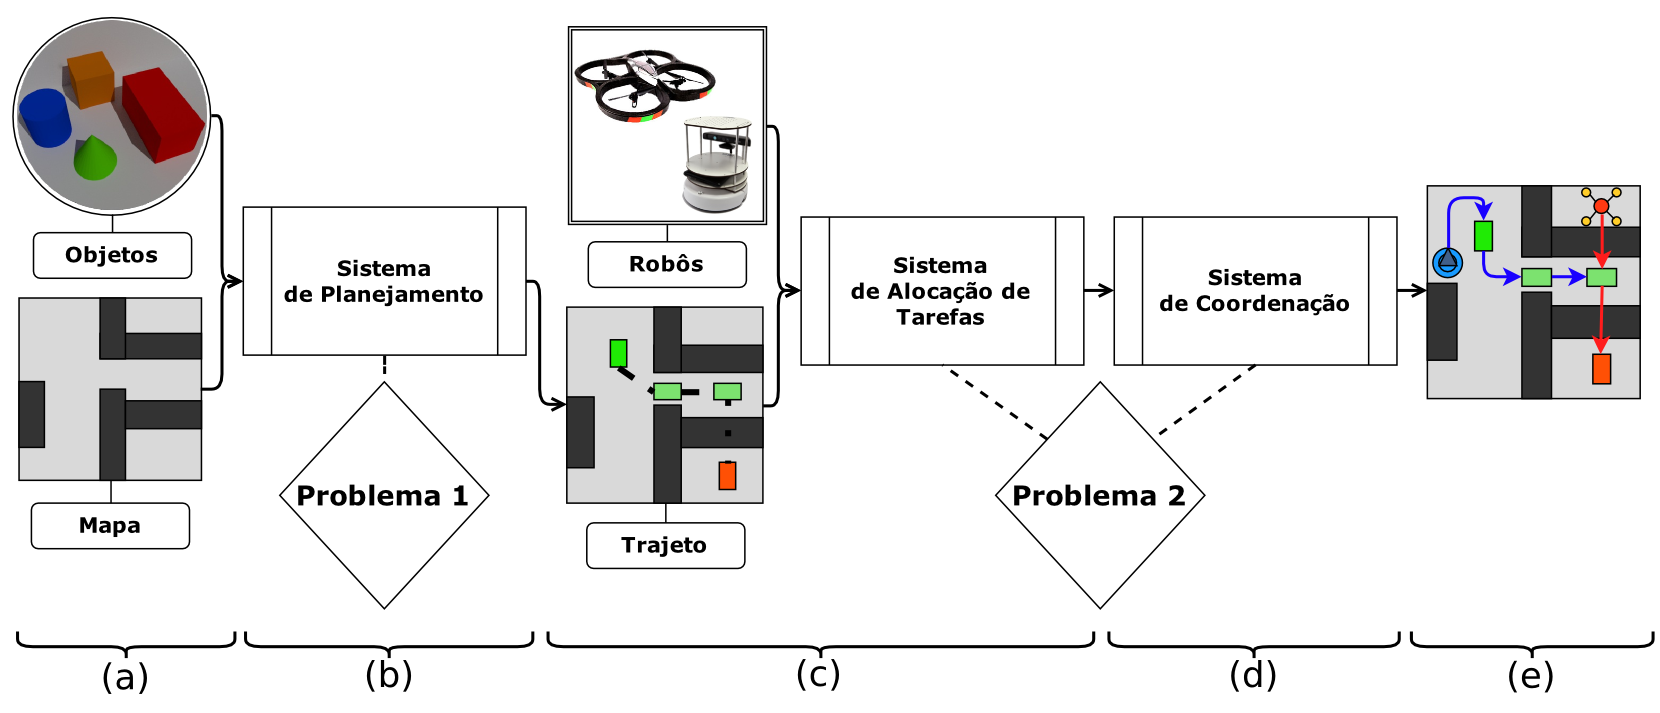
\includegraphics[width=1\textwidth]{img/001-DiagramaGeral2.png}
  \caption[Diagrama geral da Metodologia do trabalho]{Diagrama da organização do sistema apresentado, ilustrando as etapas desenvolvidas durante o processo de transporte de objetos por um time de agentes. (a) descrição do ambiente de trabalho, (b) planejamento de caminhos dos objetos, (c) planejamento de caminhos dos agentes, (d) alocação de tarefas e (e) coordenação e execução.}
  \label{fig:diagrama_geral}
\end{figure}

% Cada etapa será detalhada nas seções a seguir.
% A Figura~\ref{fig:diagrama_geral} demonstra o fluxograma do sistema implementado, além de apontar as regiões do sistema que foram foco desta pesquisa, propondo uma solução aos problemas descritos no Capítulo ~\ref{cha:introdu_o}.

% \begin{figure}[htpb]
%   \centering
%   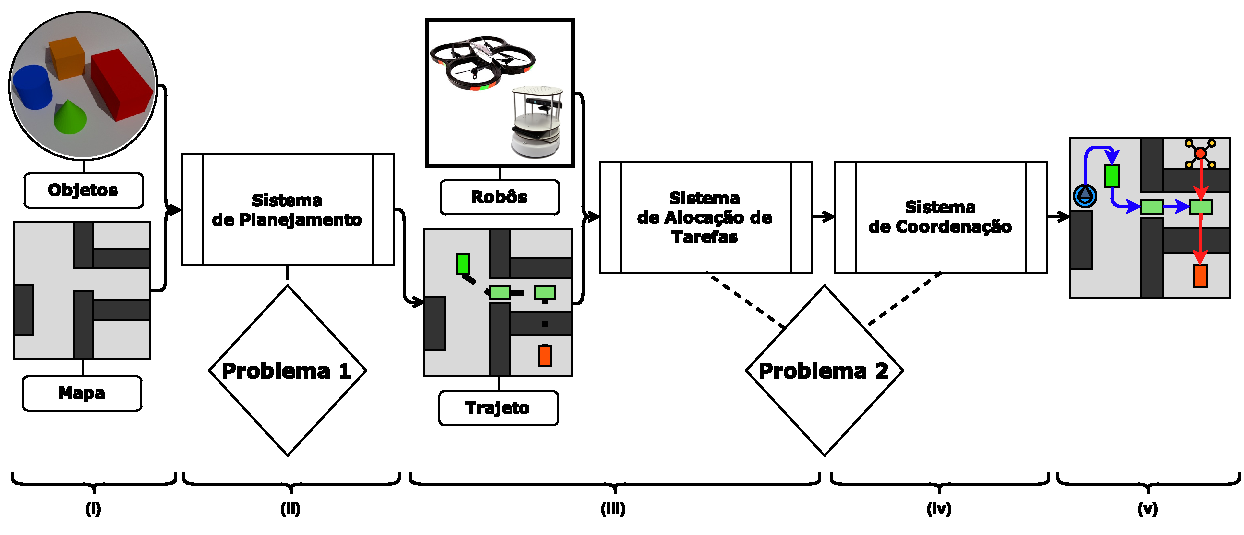
\includegraphics[width=\textwidth]{img/001-DiagramaGeral.pdf}
%   \caption[Diagrama geral da Metodologia do trabalho]{Diagrama da organização do sistema proposto, ilustrando as etapas necessárias no processo de transporte de objetos por um time de agentes.}
%   \label{fig:diagrama_geral}
% \end{figure}

% \section{Definição e Nomenclatura} % (fold)
% \label{sec:defini_o_e_nomemclatura}

% Será definido a seguir as notações utilizadas no decorrer deste trabalho:

% \subsection*{Notações da Área de Trabalho} % (fold)
% \label{sub:nota_es_da_rea_de_trabalho}

% \begin{itemize}
  % \item[\workspace]: Ambiente de trabalho utilizado na execução da tarefa de transporte definido a partir de um espaço Euclidiano $\mathbb{R}^3$ por $\workspace \subset \mathbb{R}^3$ como volume convexo;
  % \item[\obstacleset]: Conjunto \obstaclelist\ de \obstaclesetqt\ obstáculos, que serão considerados como corpos estáticos que restringem a movimentação tanto dos agentes como dos objetos a serem transportados;
  % \item[\objectset]: Conjunto \objectlist, contendo \objectsetqt\ objetos a serem transportados pelos agentes;
  % \item[\robotset]: Conjunto \robotlist, formado por \robotsetqt\ robôs disponíveis para realização da tarefa.
% \end{itemize}

% subsection nota_es_da_rea_de_trabalho (end)

% \subsection*{Notações de Funções} % (fold)
% \label{sub:nota_es_de_fun_es}

% \begin{itemize}
%   \item[\utilityfunction]: Função de utilidade utilizada na comparação de planos;
%   \item[\distancefunction]: Função de distância entre estados descritos no ambiente de trabalho \workspace. Utiliza a Distância de Manhattan;
%   \item[\timefunction]: Função que descreve a quantidade de tempo gasto para movimentação de um determinado robô \robot{i} em \workspace;
%   \item[\energyfunction]: Função que descreve a energia gasta por um agente durante a movimentação e transporte do objeto por um agente \robot{i}.
% \end{itemize}

% subsection nota_es_de_fun_es (end)

% \subsection*{Notações de Planejamento} % (fold)
% \label{sub:nota_es_de_planejamento}

% \begin{itemize}
  % \item[\movementset]: Conjunto \movementslist\ com todos os movimentos que tanto os objetos quanto os agentes conseguem realizar em \workspace;
  % \item[\movementaction]: Representa uma ação do conjunto \movementset;
  % \item[\node]: Estrutura que agrupa as características de movimentação: \nodedata, descritos a seguir:
  %   \begin{itemize}
  %     \item[\currentstate]: Estado em \workspace\ que um \node\ representa;
  %     \item[\robotstate]: Estado em \workspace\ que um robô deve ocupar para realizar o movimento descrito em um \node;
  %     \item[\type{i}]: Tipo de movimento descrito no conjunto \typeset;
  %     \item[\nodeutility]: Valor de utilidade do \node\ em referência à função \utilityfunction.
  %   \end{itemize}
  % \item[\robotinitialstatei{i}]: Estado em \workspace\ que representa o estado inicial de um determinado robô \robot{i};
  % \item[\planset]: Conjunto \planlist\ contento \plansetqt\ estruturas \node, representa um plano de movimentação;
  % \item[\typeset]: Conjunto \typelist\ que descreve os tipos de movimento disponíveis durante a execução da tarefa de transporte;
  % \item[\plantypeset]: Conjunto \plantypelist\ que descreve os tipos nos quais um plano pode ser classificado durante a fase de planejamento de ações.
  % \item[\movementtypeset]: Conjunto \movementtypelist\ de tipos que um plano é classificado, diferenciando os planos de preparação dos planos de execução, referente ao transporte do objeto;
  % \item[\robotplanset]: Conjunto de planos \robotplanlist, contendo todos os planos criados na fase de planejamento dos robôs.
% \end{itemize}

% subsection nota_es_de_planejamento (end)

% \subsection*{Notações de Alocação de Tarefas e Coordenação} % (fold)
% \label{sub:nota_es_de_aloca_o_de_tarefas}

% \begin{itemize}
%   \item[\segmentpointset]: Conjunto \segmentpointlist\ de \segmentpointsetqt\ pontos de segmentação utilizados na criação do conjunto \segmentset;
%   \item[\segmentset]: Conjunto \segmentlist\ de \segmentsetqt\ segmentos criados a partir do processo de segmentação de um plano \planset;
%   \item[\originstate]: Primeiro item de um plano \planset\ ou segmento \segment{i}, determina o estado inicial;
%   \item[\targetstate]: Último item de um plano \planset\ ou segmento \segment{i}, determina o estado final.
%   \item[\executionplanset]: Conjunto \executionplanlist\ sendo \executionplansetnotation, com uma sequência de planos capazes de realizar o transporte propriamente dito, denominado \executionplanname;
%   \item[\executionplanminset]: Similar ao conjunto \executionplanset, porém contem os planos de melhor qualidade para realização do transporte;
%   \item[\allocationgraph]: Grafo utilizado na etapa de Alocação de Tarefas;
%   \item[\allocationgraphcompress]: Representação reduzida do Grafo \allocationgraph;
%   \item[\tokenset]: Conjunto \tokenlist com \tokensetqt\ \token\ utilizados durante a etapa de coordenação para assinalar a permissão de execução de uma determinada tarefa.
% \end{itemize}

% subsection nota_es_de_aloca_o_de_tarefas (end)

\section{Fundamentos e Formalização} % (fold)
\label{sec:fundamentos_e_formaliza_o}

Os problemas tratados por este trabalho compreendem todas as etapas necessárias para a manipulação de objetos em um determinado ambiente mediante o uso de uma equipe de agentes robóticos.
Esta problemática pode ser formalmente definida como:

\begin{quotation}
  Dado um ambiente conhecido em um espaço euclidiano \environment, é definido por $\sy{workspace} \subset \environment$ um poliedro convexo como o ambiente de trabalho.
  Este espaço é discretizado em uma matriz, possuindo células \sy{cell} de tamanho unitário.

  % de três dimensões
  % Qualquer posição dentro de \sy{workspace} pode ser expressada por uma tupla com valores $(x, y, z)$, que identificam a célula \sy{cell} dentro da matriz.

  Inseridos em \sy{workspace}, são descritos os conjuntos: (i) conjunto $\sy{objectlist} = \objectlistdef$ contendo \objectsetqt\ objetos que devem ser transportados para seus respectivos destinos, (ii) conjunto $\sy{obstaclelist} = \obstaclelistdef$, no qual são representados demais objetos no ambiente de trabalho considerados como obstáculos durante a movimentação tanto dos agentes quanto dos objetos, e (iii) conjunto $\sy{robotlist} = \robotlistdef$ possuindo \robotsetqt\ robôs heterogêneos utilizados no processo de manipulação dos objetos em \sy{objectlist}.
\end{quotation}

A solução aqui descrita possui algumas limitações, casos que não foram tratados ou fogem do escopo da técnica, desta maneira, as seguintes suposições foram adotadas durante o desenvolvimento:

\begin{enumerate}
  \item Os agentes tem ciência da sua própria localização, dos objetos e dos obstáculos no ambiente;
  \item Não existirão dentro do ambiente de trabalho \sy{workspace} demais corpos capazes de se mover sozinhos além dos agentes;
  \item Existe um canal de comunicação entre os agentes, e o mesmo não possui falhas;
  \item Todos os objetos a serem transportados são iguais e de dimensões conhecidas.
\end{enumerate}

Estas suposições foram necessárias para tornar o problema tratável no sentido de focar os esforços de pesquisa e implementação especificamente na resolução da questão principal de coordenação dos agentes.

O conjunto \sy{robotlist} dos robôs utilizados será a união de dois conjuntos menores formados por tipos diferentes de agentes.
Estes tipos são definidos como:
(i) robô terrestre (\emph{\typeland}) -- agente capaz de se movimentar utilizando um sistema diferencial de locomoção, e não possuindo nenhum artefato para manipulação do objeto, que utiliza seu próprio corpo para aplicar a técnica de transporte não-preênsil \emph{PUSH},
(ii) robô aéreo (\emph{\typeaerial}) -- agente capaz de voar utilizando qualquer configuração que o permita pairar sobre um determinado ponto no espaço, como os modelos em formato de helicóptero, tricóptero ou quadcóptero, para transporte o mesmo utilizará a estratégia preênsil \emph{GRASP} para segurar o objeto e transportá-lo.
Ambos os tipos são definidos no conjunto \typelist.

O ambiente de trabalho \sy{workspace}, que em essência é um ambiente contínuo, será discretizado espacialmente através da criação de uma matriz de 3 dimensões.
As células desta matriz possuem tamanho unitário, e serão tratadas como a unidade básica de deslocamento e localização, ou seja, qualquer item no ambiente (robôs, objetos e obstáculos) ocupa no máximo 1 célula por vez, e uma determinada célula só pode ser ocupada por 1 item em um determinado tempo.
Como será descrito a seguir, todos os planos de movimentação dentro do ambiente compreenderão o deslocamento entre uma série de células, e o tamanho de um determinado plano será a sumarização de quantas células são percorridas durante sua execução.
Cada célula \sy{cell} é representada por uma tupla com valores $(x, y, z)$.

Considerando que o objetivo do trabalho apresentado é estudar e criar planos de movimentação que, uma vez executados, culminem no transporte de todos os objetos do ambiente, para uma melhor apresentação desta solução é definida uma nomenclatura relacionada ao sistema de planejamento:

\begin{description}
  \item[\sy{movementset}]: Conjunto de ações \movementslist\ que podem ser desempenhadas pelos agentes. Cada ação é representada pelo símbolo \sy{movementaction}, e algumas destas só podem ser executados por um tipo específico de agente, por exemplo, somente o agente de tipo aéreo pode executar as ações $<$\movementup, \movementdown$>$.
  \item[\sy{plan}]: Estrutura que descreve informações sobre os passos de um plano \sy{planset}. Contém uma referência para uma célula $\sy{cell} \in \sy{workspace}$, além de outros de dados que são utilizados durante a etapa de planejamento, como o tipo de agente que executará a ação \sy{movementaction}\ e um valor de utilidade (descrito na seção \ref{sub:fun_o_de_avalia_o}).
  Esta estrutura pode possuir duas notações especiais: (i) \originstate\ -- quando é o primeiro elemento do plano, e (ii) \targetstate\ -- quando é o último elemento.
  % Estrutura que descreve informações sobre uma célula \wcell, além de dados que são utilizados durante a etapa de planejamento de caminhos, como a distância entre \wcell\ e a posição final \wcell{f} que deve ser alcançado pelo plano e o valor de utilidade (descrito na seção \ref{sub:fun_o_de_avalia_o}).
  \item[\sy{planset}]: Plano \planlist\ que descreve uma sequência de estruturas \sy{plan}. Somente através desta sequência é possível registrar quais ações são necessárias para realização da movimentação. Por exemplo, para realizar a movimentação da célula \wcelli{1} (5, 5, 1) para \wcelli{2} (5, 6, 1), deve ser executada a ação \movementactioni{3}\ $<\movementforward>$.
  \item[\sy{executionplanset}]: Conjunto de planos \planset, nomeado plano de execução, que descreve todos as trajetórias a serem executadas pelos agentes para realizar o transporte de todos os objetos em \objectset.
\end{description}

Objetivamente, durante as etapas de planejamento, é desejável encontrar os melhores planos, isto é, aqueles com a melhor combinação de ações, capazes de movimentar um determinado objeto de sua posição atual até um ponto de destino.
Para tal, foi desenvolvido uma função de utilidade (descrita na seção \ref{sub:fun_o_de_avalia_o}) utilizada para quantificar um determinado plano, utilizada para comparar distintos planos quanto à sua qualidade.
Desta maneira, o conjunto de planos \sy{executionplanset}, é aquele contendo os planos necessários para o transporte de todos os objetos minimizando o custo total das ações.
% Desta maneira, o conjunto de planos \sy{executionplanset} a serem executados durante o transporte deve ser aquele que siga a seguinte notação:
% O conjunto de planos que descrever a minimização total da utilidade, será aquele que será executado para o transporte dos objetos.

\subsection{Notação gráfica} % (fold)
\label{sub:nota_o_gr_fica}

Como o sistema desenvolvido compreende um ambiente de trabalho no qual diversos componentes estão disposto espacialmente no mesmo, para um melhor entendimento do processo desenvolvido, alguns diagramas foram desenvolvidos, demonstrando os casos estudados nesta metodologia, possuindo uma série de elementos gráficos.
% Estes servirão para ilustrar os procedimentos criados nesta metodologia.
A seguir é listado todos os elementos utilizados:

\begin{table}[h]
    \centering
    \begin{tabular}{|c|l|}
    \hline
    Figura & Descrição \\
    \hline
    \raisebox{-0.8\height}{ \img{robot_land.pdf}{2.5em} } & \raisebox{-1.6\height}{ Figura representativa de um robô terrestre; } \\[2em]
    \hline
    \raisebox{-0.8\height}{ \img{robot_aerial.pdf}{2.5em} } & \raisebox{-1.6\height}{ Figura representativa de um robô aéreo; } \\[2em]
    \hline
    \raisebox{-0.8\height}{ \img{object_start.pdf}{2.5em} } & \raisebox{-1.6\height}{ Figura representativa da posição inicial de um objeto; } \\[2em]
    \hline
    \raisebox{-0.8\height}{ \img{object_end.pdf}{2.5em} } & \raisebox{-1.6\height}{ Figura representativa da posição final de um objeto; } \\[2em]
    \hline
    \raisebox{-0.8\height}{ \img{obstacle.pdf}{2.5em} } & \raisebox{-1.6\height}{ Figura representativa de um obstáculo; } \\[2em]
    \hline
    \raisebox{-0.8\height}{ \img{StateFigure.pdf}{2.5em} } & \raisebox{-1.6\height}{ Figura representativa de uma célula no ambiente de trabalho; } \\[2em]
    \hline
    \raisebox{-0.8\height}{ \img{PlanFigure.pdf}{2.5em} } & \raisebox{-1.6\height}{ Figura representativa de um plano; } \\[2em]
    \hline
    \end{tabular}
    \caption{Descrição dos elementos utilizados nos diagramas de exemplificação.}
    \label{table:graphic_elements}
\end{table}

% \begin{figure}[htpb]
%   \centering
%   \setlength{\fboxsep}{0pt}
%   \begin{subfigure}[t]{0.45\textwidth}
%     \centering
%     \fbox{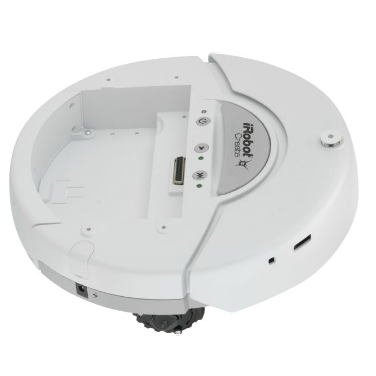
\includegraphics[height=0.25\textheight]{img/irobot_create.png}}
%     \caption{}
%     \label{fig:robos_casa_a}
%   \end{subfigure}%
%   \hspace{0.02cm}
%   \begin{subfigure}[t]{0.45\textwidth}
%     \centering
%     \fbox{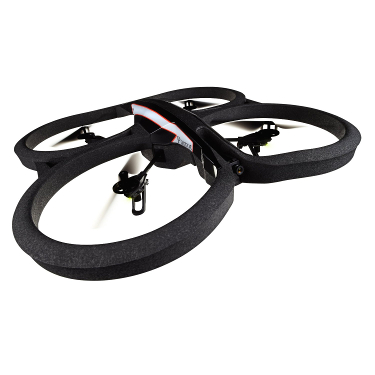
\includegraphics[height=0.25\textheight]{img/ar_drone.jpg}}
%     \caption{}
%     \label{fig:robos_reais}
%   \end{subfigure}
%   \caption[Plataformas robóticas reais utilizadas para o transporte de objetos]{(a) iRobot Create -- robô terrestre com sistema diferencial de movimentação, (b) Parrot AR-Drone -- robô aéreo no formato quadrotor.}
%   \label{fig:robos_casa}
% \end{figure}


% section nota_es (end)

\section{Função de Utilidade} % (fold)
\label{sub:fun_o_de_avalia_o}

Durante o processo de planejamento de caminhos do objeto, de modo a considerar a heterogeneidade dos agentes, são analisadas características relacionadas ao tipo de robô que pode executar o plano, de modo a encontrar aquele que melhor satisfaça as necessidades do sistema.

Para tal, são avaliados dois parâmetros para cada tipo agente, estes descrevem a utilidade da execução de um determinada ação \sy{movementaction} dentro de um plano \sy{planset}, de modo a quantificar esta ação em um aspecto passível de ser comparado.
As características a seguir são utilizadas na avaliação:

\begin{itemize}
  \item \textbf{Tempo de deslocamento}:
    Tempo necessário para movimentação entre células \sy{cell}. Este aspecto está relacionado à velocidade média que um determinado robô consegue realizar o deslocamento. Descrito pela função \sy{timef};
  \item \textbf{Custo de deslocamento}:
    Custo para movimentação entre células \sy{cell}. Para cada tipo de robô utilizado no transporte, é calculado o gasto médio de energia que o mesmo tem durante o deslocamento. Descrito pela função \sy{energyf}.
\end{itemize}

Formalmente, a Equação \ref{eq:util_function} descreve a função de utilidade \sy{utilityf}, que avalia um determinado tipo de agente $\type{i} \in \typelist$, dando-lhe uma pontuação baseado em seus atributos. O valor gerado desta análise é utilizado para guiar a criação do plano de movimentação do objeto (descrito na Seção \ref{sub:planejamento_de_caminhos_objeto}).

\begin{equation}
  \sy{utilityf}(\type{i}, \movementaction) = \alpha \cdot \sy{timef}(\type{i}) + (1-\alpha) \cdot \sy{energyf}(\type{i}).
  \label{eq:util_function}
\end{equation}

As constantes definidas por $<\alpha>\ =\{\alpha \in \mathbb{R} | 0 \leq \alpha \leq 1\}$ são utilizadas como fatores de ponderação entre as características avaliadas de forma a refletir a priorização de certas atividades, como executar no menor tempo possível ou com a menor energia gasta, por exemplo.
Este modelo é flexível pois pode ser reconfigurado para atender a diversas necessidades, além de adicionar ao planejamento particularidades de cada agente. O valor resultante desta função é utilizado como parte da heurística utilizada na busca pelo melhor plano de movimentação.

Para determinar o valor de utilidade de um determinado plano \sy{planset}, os valores de utilidade de cada \sy{plan}\ que o constitui são somados como demonstrado na Equação \ref{eq:plan_util_function}:

\begin{equation}
  \sy{utililityplanf}(\sy{planset}) = \displaystyle\sum_{\sy{plan} \in \sy{planset}} \sy{utilityf}(k(\sy{plan})).
  \label{eq:plan_util_function}
\end{equation}

Considerando que a função de utilidade está baseada no tipo \type{i} de um agente que realizará uma determinada ação \movementaction, é definida a equação \ref{eq:get_data}, que extrai tais informações diretamente de uma estrutura \sy{plan}, como definida a seguir:

\begin{equation}
  k : \sy{plan} \mapsto \type{i}, \movementaction.
  \label{eq:get_data}
\end{equation}

A função de utilidade \sy{utilityf} juntamente com a equação \ref{eq:plan_util_function}, é utilizada para determinar, dentre os diversos planos de movimentação que podem ser criados, qual o melhor plano, ou seja, aquele que possuir o menor custo total para realização das ações.
Neste sentido, a metodologia apresentada visa encontrar o conjunto \sy{executionplanset}, aquele que minimize o custo total de todo o sistema.
A equação \ref{eq:min_plan} ilustra este objetivo.

\begin{equation}
  \arg\min_{\executionplanset} \sum_{\substack{\planset \in \executionplanset}} \sy{utililityplanf}(\sy{planset}).
  \label{eq:min_plan}
\end{equation}

% A comparação entre planos é aplicada quando existem mais de um plano para realizar a movimentação entre duas mesmas células \sy{cell}, e ao considerar as dimensões analisadas (tempo e energia), objetiva-se realizar a minimização das mesmas, portanto, ao comparar planos, aquele com o menor valor de utilidade será escolhido como melhor.

% subsection fun_o_de_avalia_o (end)

\section{Planejamento de Caminhos - Objeto} % (fold)
\label{sub:planejamento_de_caminhos_objeto}

A primeira etapa da técnica apresentada é a criação de planos de movimentação para cada objeto $\object{i} \in \sy{objectlist}$, este processo é dividido em dois estágios: (i) planejamento de caminhos e (ii) segmentação do plano.
% Este último passo servirá de base para realização do planejamento de caminhos dos agentes e alocação de tarefas.
Para realização do planejamento, assume-se que o objeto a ser transportado é capaz de movimentar-se dentro da área de trabalho \sy{workspace}.
Os movimentos disponíveis para o objeto nesta fase estão listados no conjunto \sy{movementset}.

% ALGORITMO DE PLANEJAMENTO DE CAMINHOS

\subsection{Planejamento} % (fold)
\label{sub:planejamento}

% subsection planejamento (end)

O algoritmo implementado é uma variação do Algoritmo A* (\cite{Hart1968}), como é descrito no Algoritmo \ref{alg:a_start_algorithm}.
Inicialmente é criado um grafo direcionado vazio denominado \sy{plangraph}, que guardará referências para todas as estruturas \sy{plan} que foram exploradas enquanto a busca pelo plano é executada.
Além disso, seguindo a mesma estratégia do algoritmo, é criada uma lista nomeada \sy{fringe}, que guarda as referências para todos os nós folhas do grafo \sy{plangraph}, ou seja, todas as estruturas \sy{plan} que ainda não foram exploradas e se encontram na borda da área de busca.

\begin{algorithm}[htpb]
  \caption[AStar]{AStar(\originstate, \targetstate, \sy{movementset}, \sy{workspace})}
  \label{alg:a_start_algorithm}
  \begin{algorithmic}[1]

  \STATE{$\plangraph \leftarrow \emptyset$}
  \STATE{$\fringe \leftarrow \{\originstate\}$}
  \STATE{}
  \STATE{$\originstate[utility] \leftarrow \utilityfunction(\originstate) + \text{distance}(\originstate, \targetstate)$}

  \STATE{}
  \WHILE{$\fringe \neq \emptyset$}

    \STATE{// vertex selection step}
    % \STATE{$\plan{j} \leftarrow \{ \forall \plan{i} \in \fringe : \text{min}\ \plan{i}[utility] \}$}
    \STATE{$\plan{j} \leftarrow \min(\fringe)$}

    \STATE{}
    \IF{$\plan{j} = \targetstate$}
      \RETURN{reconstruct\_path(\plan{j})}
    \ENDIF

    \STATE{}
    \STATE{$\fringe \leftarrow \fringe \setminus \{\plan{j}\} $}
    \STATE{$\plangraph \leftarrow \plangraph \cup \{\plan{j}\}$}
    \STATE{}

    \STATE{// expansion step}
    \STATE{expansion\_algorithm(\plan{j}, \targetstate, \movementset, \fringe, \plangraph, \workspace)}

    % \FORALL{$\movementaction \in \movementset$}
    %   \STATE{$\nextstate \leftarrow \{ \text{move} : \plan{w}, \movementactioni{x} \mapsto \plan{z}\ |\ \text{move}(\plan{i}, \movementaction) \}$}
    %   \STATE{}
    %   \IF{$\nextstate \in \plangraph$}
    %     \STATE{continue}
    %   \ENDIF
    %   \STATE{}
    %   \STATE{$\nextstate[utility] \leftarrow \utilityfunction(\nextstate)$}
    % \ENDFOR

  \ENDWHILE

  \RETURN{\FALSE}

  \end{algorithmic}
\end{algorithm}

Uma etapa necessária durante a execução deste algoritmo é a seleção do melhor vértice a ser expandido (linha 8 do Algoritmo \ref{alg:a_start_algorithm}), para tal, é considerada como heurística de seleção dois valores: (i) a distância remanescente estimada entre a célula \sy{cell} referenciada por \sy{plan} e a célula de destino do plano -- utiliza-se a distância de Manhattan; e (ii) o valor de utilidade calculado para \sy{plan}, considerando o tipo de agente que pode realizar a ação.
Estes valores são somados, resultando no valor de utilidade da estrutura \sy{plan} para cada tipo de agente.
Para garantir que o plano siga por um caminho sempre tentando minimizar o valor de custo total, aquela que possuir a menor pontuação, independente de tipo, será escolhida para expansão.
Esta operação ocorre considerando os elementos do conjunto \sy{fringe}.

O Algoritmo \ref{alg:expansion} descreve o processo de expansão de um determinado vértice do grafo \sy{plangraph} (linha 19 do Algoritmo \ref{alg:a_start_algorithm}).
As demais etapas do algoritmo A*, como a construção do caminho desde a origem até o destino do plano, são similares à implementação original do mesmo.
O passo de expansão garante que todas as ações possíveis de serem realizadas a partir de uma determinada posição em \sy{workspace} possam ser posteriormente avaliadas pela função de seleção.

\begin{algorithm}[htpb]
  \caption[ExpansionAlgorithm]{ExpansionAlgorithm(\currentstate, \targetstate, \sy{movementset}, \sy{fringe}, \sy{plangraph}, \sy{workspace})}
  \label{alg:expansion}
  \begin{algorithmic}[1]

    % \STATE{\currentstate\ $\leftarrow$ select\_state\_from(\fringe)}
    % \STATE{$\plangraph \leftarrow \plangraph \cup \{\currentstate\}$}
    \STATE{$\wcell \leftarrow$ get\_position(\currentstate)}

    \FORALL{\movementaction\ $\in$ \movementset}

      \STATE{}
      \STATE{$\wcell' \leftarrow$ apply\_action(\movementaction, \wcell)}
      \STATE{$\robotstate \leftarrow$ is\_executable(\movementaction, \wcell')}
      \STATE{$\nextstate \leftarrow$ create\_struct(\currentstate, \wcell', \movementaction)}
      \STATE{$\nextstate[utility] \leftarrow \utilityfunction(\nextstate) + \text{distance}(\nextstate, \targetstate)$}
      \STATE{}

      \IF{\nextstate\ $\in$ \plangraph\ \OR is\_colliding(\workspace, \nextstate) \OR \NOT \robotstate}
        \STATE{$\plangraph \leftarrow \plangraph \cup \{\nextstate\}$}
        \STATE{\textbf{continue}}
      \ENDIF

      \STATE{}
      \STATE{$\fringe \leftarrow \fringe \cup \{\nextstate\}$}
    \ENDFOR
  \end{algorithmic}
\end{algorithm}

Durante a etapa de expansão, um vértice do grafo de busca é modificado de forma a verificar quais ações podem ser realizadas a partir do mesmo.
Baseado na referência para a célula \wcell\ da estrutura \currentstate, conseguida através da função \emph{get\_position()}, o algoritmo cria novas referências de células aplicando todas as ações $\movementaction\ \in \movementset$ (função \emph{apply\_action()}).
Uma vez com esta posição, a função \emph{is\_executable} considera se a ação é possível de ser executada, no caso, se a posição \robotstate, na qual o agente deve estar para realizar a ação, não colide com outros obstáculos, robôs ou objetos.
Possuindo estes dados, é criado um novo vértice \nextstate, que guarda informações sobre a ação utilizada para chegar ao mesmo, além do parentesco com a estrutura \currentstate\ (função \emph{create\_struct()}).

Um processo importante que é realizado durante a criação do novo vértice é a execução do cálculo de utilidade do mesmo, que ocorre similar ao representado na linha 4 do Algoritmo \ref{alg:a_start_algorithm}. Além deste cálculo, é aplicada uma penalização no custo sempre que a ação que resultou a criação do vértice for diferente da ação do vértice pai.
Esta penalização proporciona a criação de planos com a menor quantidade de mudanças de direção possível, bastante importante, principalmente no transporte terrestre, pois o agente não necessita realizar mais deslocamentos para empurrar o objeto para outras direções.

Dispondo destes resultados, o algoritmo testa se a nova posição assinalada já foi estudada anteriormente (se está presente em \plangraph), se a mesma colide com algum obstáculo do ambiente (função \emph{is\_colliding()}) e se não é possível de ser executada. Se algum destes testes for positivo, esta nova estrutura \nextstate\ é considerada como inválida e adicionada diretamente ao grafo de vértices já estudados, caso contrário, o mesmo será adicionado ao conjunto \fringe, para uma posterior expansão.

O algoritmo de exploração termina em dois casos, (i) quando o conjunto \sy{fringe}\ está vazio, indicando que não existe um caminho até o estado de destino \targetstate, ou (ii) quando o estado selecionado para expansão é o estado final, neste caso, é reconstruído o caminho desde o destino, utilizando as informações de parentes de vértices, até a posição de origem.
O resultado do algoritmo de exploração é um plano \sy{planset}, que pode ser visto como um sub-grafo de \sy{plangraph}.
A Figura \ref{fig:object_plan} mostra um planejamento de exemplo para um objeto dentro de um certo ambiente.
Uma vez que o plano seja criado, o passo de segmentação é executado.

Como o algoritmo implementado é uma variação do Algoritmo A*, o mesmo possui uma complexidade similar, relacionado a dois fatores:
(i) a organização do conjunto \sy{fringe} para escolha do vértice a ser expandido, que no pior caso possui complexidade $\mathcal{O}(n^k)$, na qual $n$ é o número de vértices explorados durante a busca pelo caminho, e $k$ é a quantidade de possíveis ações que podem ser tomadas durante o processo, no caso $k=|\sy{movementset}|= 6$.
% possuindo uma complexidade de $\mathcal{O}(n log(n))$, na qual $n$ é o tamanho do conjunto, e
(ii) o tempo necessário para computar o valor da heurística de utilidade, que neste caso é $\mathcal{O}(1)$.

% ALGORITMO DE SEGMENTAÇÃO DO PLANO

\subsection{Segmentação} % (fold)
\label{sub:segmenta_o}

A segmentação tem sua importância no transporte terrestre pois, considerando que os robôs terrestres só possuem a capacidade de empurrar os objetos, sempre que há uma mudança na direção do movimento, o robô deve realizar a ação de \emph{PUSH} por outro lado objeto, e neste momento, existe a possibilidade de que um agente diferente seja mais apto, com uma melhor utilidade para realizar a ação, que o robô que está atualmente realizando a tarefa.
Em relação à mudança de tipo de movimento, passando de \emph{PUSH} para \emph{GRASP}, a segmentação do plano consegue destacar esta diferença, e facilitar o tratamento posteriormente.

O processo de segmentação executa a divisão do plano \sy{planset} criado pelo algoritmo de busca, gerando o conjunto \sy{segmentset}\ como resultado da operação.
Este conjunto será utilizado durante a etapa de planejamento dos robôs e posteriormente para alocação de tarefas entre os agentes.

Para realizar a segmentação do plano, são executados dois algoritmos:
(i) algoritmo de criação dos pontos de segmentação (Algoritmo \ref{alg:segment_point_creation}), no qual é criado um conjunto auxiliar, nomeado \segmentpointset, contendo uma lista de tuplas, cada uma destas assinalando uma mudança de direção dentro do plano, e
(ii) algoritmo de criação dos segmentos (Algoritmo \ref{alg:segment_creation}), que utiliza a lista de referências em \segmentpointset\ para criar uma lista de segmentos do plano.

\begin{algorithm}
  \caption[SegmentPointSetCreation]{SegmentPointSetCreation(\sy{planset}, \segmentpointset)}
  \label{alg:segment_point_creation}

  \begin{algorithmic}[1]

  \FORALL{$\currentstate_{i}, \currentstate_{i+1} \in \planset$}

    \IF{ is\_aerial($\currentstate_{i}$) \AND is\_aerial($\currentstate_{i+1}$)}
      \STATE{\textbf{continue}}
    \ENDIF

    \STATE{$\movementactioni{i} \leftarrow$ get\_action($\currentstate_{i}$)}
    \STATE{$\movementactioni{i+1} \leftarrow$ get\_action($\currentstate_{i+1}$)}

    \IF{$\movementactioni{i} <> \movementactioni{i+1}$}
      \STATE{$\segmentpoint{i} \leftarrow$ create\_segment\_point($\currentstate_{i}$, $\currentstate_{i+1}$)}
      \STATE{$\segmentpointset \leftarrow \segmentpointset \cup \{\segmentpoint{i}\}$}
    \ENDIF
  \ENDFOR

  \RETURN{\segmentpointset}

  \end{algorithmic}
\end{algorithm}

\begin{algorithm}
  \caption[SegmentSetCreation]{SegmentSetCreation(\segmentpointset, \sy{segmentset}, \originstate, \targetstate)}
  \label{alg:segment_creation}

  \begin{algorithmic}[1]

    \FORALL{\segmentpoint{i} $\in$ \segmentpointset}
      \STATE{$\currentstate_{0} \leftarrow \segmentpoint{i}[0]$}
      \STATE{$\currentstate_{1} \leftarrow \segmentpoint{i}[1]$}

      \IF{$\segmentset = \emptyset$}
        \STATE{$\segment{i} \leftarrow$ create\_segment(\originstate, $\currentstate_{0}$)}
      \ELSE
        \STATE{$\segment{i} \leftarrow$ create\_segment($\currentstate_{temp}$, $\currentstate_{0}$)}
      \ENDIF
      \STATE{$\currentstate_{temp} \leftarrow \currentstate_{1}$}
      \STATE{$\segmentset \leftarrow \segmentset \cup \{\segment{i}\}$}
    \ENDFOR
    \STATE{$\segment{i} \leftarrow$ create\_segment($\currentstate_{temp}$, \targetstate)}
    \STATE{$\segmentset \leftarrow \segmentset \cup \{\segment{i}\}$}

    \RETURN{\segmentset}

  \end{algorithmic}
\end{algorithm}

O processo de criação dos pontos de segmentação (Algoritmo \ref{alg:segment_point_creation}), percorre par a par os elementos de um determinado plano \sy{planset}, primeiramente observando se ambas as estruturas representam posições aéreas (função \emph{is\_aerial()}), se o teste for positivo, então não há necessidade de criar um ponto de segmentação, pois o transporte aéreo, diferente do terrestre, não pode ser interrompido durante sua execução, independente de quantas vezes troque de direção; após o teste, é requisitado das estruturas as ações utilizadas para a sua criação (função \emph{get\_action()}), pois sempre que estas ações forem diferentes, uma mudança de direção ocorreu, ocasionando na criação de um novo ponto de segmentação (função \emph{create\_segment\_point()}), posteriormente adicionado ao conjunto \segmentpointset.
Cada ponto de segmentação é uma tupla com dois valores, referenciando ambas estruturas ($\currentstate_{i}$, $\currentstate_{i+1}$).

Em continuação, é executado o Algoritmo \ref{alg:segment_creation}, que toma como base o conjunto auxiliar \segmentpointset\ para criar os segmentos. O algoritmo itera sobre todos os pontos de segmentação, criando segmentos do plano \sy{planset} (função \emph{create\_segment()}).
Após este processo, o conjunto \segmentlist\ é criado, possuindo \segmentsetqt\ segmentos, cada um destes é um sub-plano do plano original \sy{planset} e denominam trajetos do plano que: (i) se for terrestre, não possui nenhuma mudança de direção, e (ii) se for aéreo, se estende desde o passo no qual é assinalada a decolagem, até o passo onde um pouso é descrito.
Similar ao plano \sy{planset}, cada segmento \segment{i} no conjunto \sy{segmentset} também possui referências para os estados \originstate\ e \targetstate, com a mesma definição. Na Figura \ref{fig:object_plan} podem ser observados os segmentos que foram criados para o plano de um objeto de teste.

A criação dos pontos de segmentação demonstrada no Algoritmo \ref{alg:segment_point_creation}, como é baseado exclusivamente na quantidade de passo do plano, possuindo uma complexidade de $\mathcal{O}(n)$, onde $n$ é o tamanho do plano. Já o Algoritmo \ref{alg:segment_creation} possui similar complexidade de $\mathcal{O}(m)$, porém $m$ é a quantidade de elementos do conjunto \segmentpointset.

% Pode ser observado que a movimentação em meio aéreo não segmentado, mesmo que mude de direção diversas vezes.
% Esta restrição é aplicada pois uma vez que um robô inicie o transporte aéreo, não é possível que um agente diferente continue o transporte no ar, de modo que a troca de agentes é permitida somente quando o objeto é depositado.

\begin{figure*}[ht!]
  \centering
  \setlength{\fboxsep}{0pt}
  \fbox{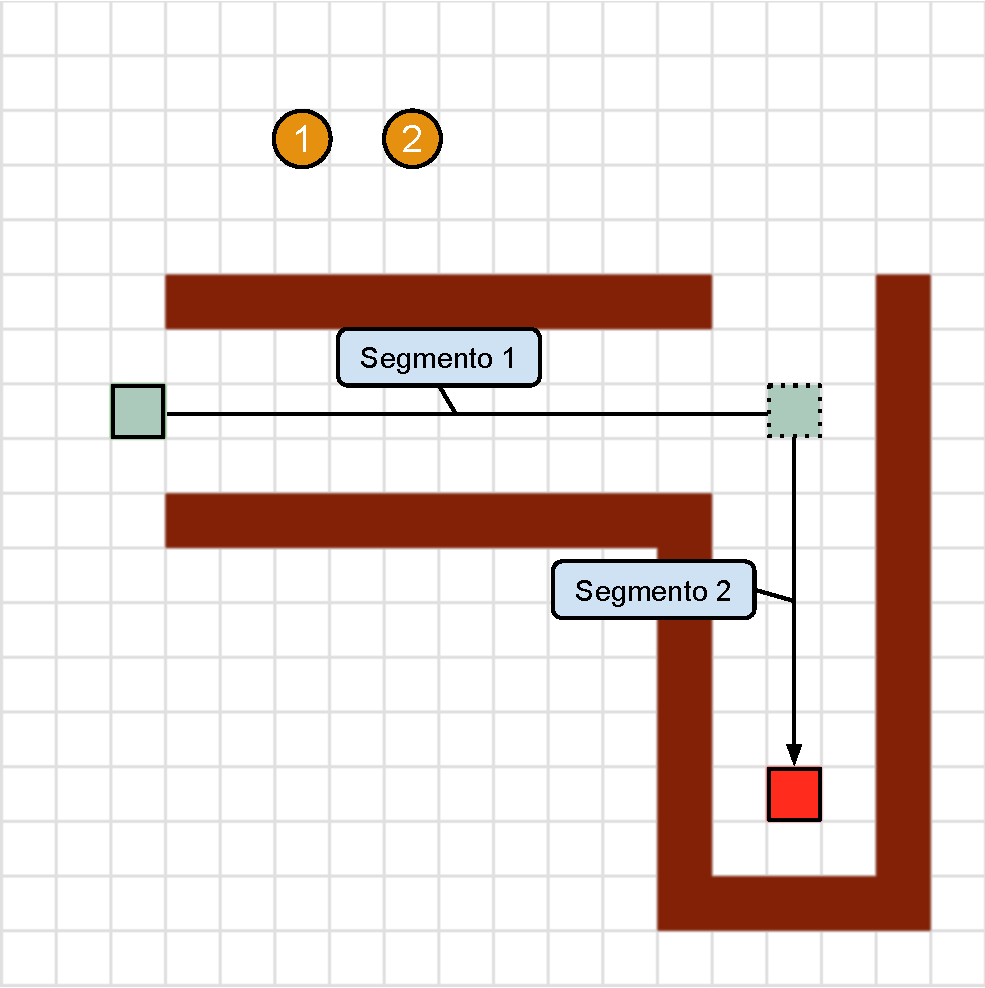
\includegraphics[height=0.45\textheight]{img/ObjectMovement1.pdf}}
  \caption[Planejamento e Segmentação do plano de movimentação de um objeto]{Etapa de Planejamento de caminhos e Segmentação do plano de um objeto a ser transportado em um ambiente de teste. O exemplo ilustra o plano de um objeto, a criação de dois segmentos, pois há somente uma troca de direção em seu plano. Como não existem agente aéreos no ambiente, somente um trajeto terrestre foi planejado.}
  \label{fig:object_plan}
\end{figure*}

% subsection planejamento_de_caminhos_objeto (end)

\section{Planejamento de Caminhos - Agentes} % (fold)
\label{sub:planejamento_de_caminhos_agentes}

Esta etapa visa a criação de planos de movimentação para os agentes, de modo a provê-los do melhor trajeto para se locomover dentro do ambiente.
Planos estes utilizados nos casos onde o agente deve se aproximar do objeto e posteriormente, indicar a rota de transporte.
Dentro do sistema, estes planos serão utilizados tanto na fase de alocação de tarefas quanto na execução do transporte.

% pois, além do tipo de agente, é também através deles que é possível realizar a comparação entre dois agentes que pretendem transportar o mesmo objeto.
% A etapa de planejamento dos agentes envolve a criação de planos que indiquem a melhor rota a ser executada para que cheguem em um determinado ponto do mapa.
% Este algoritmo é utilizado tanto

O planejamento da movimentação de cada robô $\robot{i} \in \sy{robotlist}$ ocorre de maneira iterativa, de modo que os planos são gerados no decorrer da fase de alocação de tarefas (Seção \ref{sec:aloca_o_de_tarefas}).
Cada plano possui um valor de utilidade mediante a função \sy{utililityplanf}\ descrita na Equação \ref{eq:plan_util_function} que quantifica sua qualidade em relação aos demais planos.
Estes valores serão utilizados para escolher o melhor agente para realizar um determinado segmento do transporte.

Para criar um plano para um determinado agente, é utilizado um algoritmo similar ao utilizado para criação dos planos para os objetos (algoritmos \ref{alg:a_start_algorithm} e \ref{alg:expansion}), com as seguintes modificações: (i) o teste de colisão usando a função \emph{is\_colliding()} usa o corpo do robô como referência, e (ii) a função \emph{is\_executable()} não é executada, considerando que este teste só se aplica ao objeto.
Este algoritmo é adotado na criação de dois tipos de planos, listados no conjunto $\sy{movementtype} =$ \{\movementtypepremove, \movementtypemove\} e descritos a seguir:

\begin{itemize}
  \item \textbf{\movementtypepremove}: usado pelos agentes para se aproximar do objeto a ser transportado. O plano inicia-se na posição atual do robô até a posição indicada por \robotstate, que se encontra na estrutura \originstate\ do primeiro segmento ainda não realizado de um objeto alvo.
  \item \textbf{\movementtypemove}: executado quando o robô está realmente realizando o transporte. Parte da posição inicial do segmento (\originstate) até o estado final (\targetstate).
\end{itemize}

A Figura \ref{fig:robot_plan} ilustra todos os possíveis planos que os agentes podem executar a fim de realizar a tarefa de transporte, e seus respectivos tipos.
Os planos partem da posição do agente \robotinitialstate\ enumerados por agente (note que apesar do diagrama demarcar uma célula adjacente, a célula utilizada para o planejamento é a qual o agente se encontra no momento), indo até os estados \robotstate\ descritos nas estruturas \originstate\ ou \targetstate\ de cada segmentos.
Para uma melhor diferenciação, os estados \robotstate\ foram enumerados.

\begin{figure}[hbtp]
    \centering
    \setlength{\fboxsep}{0pt}
    \fbox{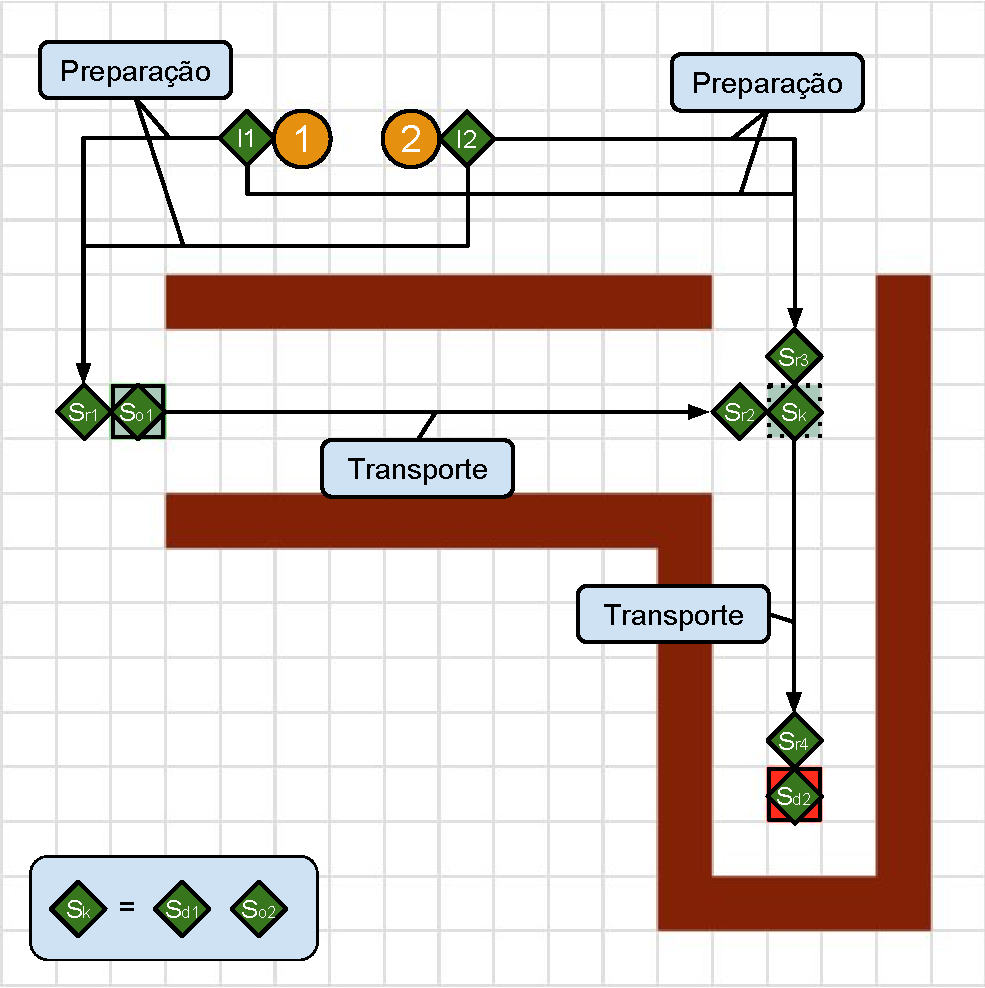
\includegraphics[height=0.45\textheight]{img/ObjectMovement2.pdf}}
    \caption[Planos de movimentação dos agentes]{Exemplo de planos gerados para os agentes que podem ser utilizados para realizar o transporte do objeto. Cada agente cria seus próprios planos baseado na quantidade e configuração de cada segmento do trajeto do objeto a ser transportado. A quantidade de planos criados cresce à medida que existem mais agentes, objetos, ou mesmo quando existem mais segmentos em um determinado plano.}
    \label{fig:robot_plan}
\end{figure}

% subsection planejamento_de_caminhos_agentes (end)

\section{Alocação de Tarefas} % (fold)
\label{sec:aloca_o_de_tarefas}

Na etapa de alocação de tarefas, o principal objetivo é determinar uma sequência de movimentos, que uma vez realizados, culminem no transporte de todos os objetos para suas respectivas posições finais, simultaneamente minimizando o custo total dos planos executados pelos agentes.

A ordem na qual os objetos serão transportados tem direta influência na distância percorridas pelos agentes, desta forma, a equipe de agentes deve analisar o estado do ambiente de trabalho (suas próprias posições e as posições dos objetos) e escolher a melhor sequência para execução, por exemplo, realizar o transporte visando os objetos mais próximos de cada agente ao invés dos mais distantes.

transportar os objetos mais próximos seja melhor que outros mais distantes.

O foco da alocação de tarefas no âmbito do transporte cooperativo de objetos é o de encontrar a melhor seleção de tarefas, ao considerar os agentes e objetos dispostos no ambiente.
Desta maneira, é apresentado um algoritmo distribuído que realiza a alocação dos segmentos entre os agentes.

A fase de planejamento de caminhos dos objetos (Seção \ref{sub:planejamento_de_caminhos_objeto}) ocorre de forma centralizada, de modo que não mudará no decorrer da execução das tarefas.
Um membro da equipe é elegido de forma arbitrária e realiza esta etapa, disponibilizando para os demais agentes os planos resultantes através de uma comunicação em \emph{broadcast}, de forma a sincronizar todos os agentes para o inicio da fase de alocação.
Munidos destas informações, toda a equipe de agentes participa da alocação de tarefas, executando o Algoritmo \ref{alg:task_allocation}.

\begin{algorithm}
  \caption[TaskAllocationProcess]{TaskAllocationProcess(\objectset)}
  \label{alg:task_allocation}

  \begin{algorithmic}[1]
    \LOOP
      \STATE{$\workobjectset \leftarrow$ build\_work\_list(\objectset)}

      \IF{$\workobjectset = \emptyset $}
        \STATE{\textbf{break}}
      \ENDIF
      \STATE{}
      \STATE{utility\_memory $\leftarrow$ \{\}}

      \FORALL{ $\object{i} \in \workobjectset$ }
        \STATE{$\segment{i} \leftarrow$ get\_first\_segment(\object{i}) }

        \STATE{$\planset_{m} \leftarrow$ create\_move\_plan(\segment{i})}
        \STATE{$\planset_{t} \leftarrow$ create\_transport\_plan(\segment{i})}

        \STATE{total\_utility $\leftarrow \sy{utililityplanf}(\planset_{m}) + \sy{utililityplanf}(\planset_{t})$}

        \STATE{utility\_memory $\leftarrow$ utility\_memory $\cup$ \{\object{i}: total\_utility\}}
      \ENDFOR
      \STATE{}

      \STATE{share\_memory(utility\_memory)}
      \STATE{wait\_until\_receive\_all\_memories()}
      \STATE{}

      \STATE{utility\_memory $\leftarrow$ utility\_memory $\cup$ get\_team\_memory()}
      \STATE{allocation $\leftarrow$ execute\_hungarian\_method(utility\_memory)}
      \STATE{update\_own\_tasks(allocation)}

      \STATE{}
      \STATE{share\_ready()}
      \STATE{wait\_until\_reveice\_all\_ready()}

    \ENDLOOP
  \end{algorithmic}
\end{algorithm}

O algoritmo demonstrado é executado por cada agente, e se torna sincronizado dentre a equipe mediante o uso das funções de espera (\textit{wait\_until\_receive\_all\_memories()} e \textit{wait\_until\_reveice\_all\_ready()}).
Internamente, para decidir qual agente é o mais apto para qual tarefa, é executado o Algoritmo de Otimização Combinatória Húngaro (\cite{Munkres1957}).

Inicialmente o algoritmo cria um subconjunto de objetos, com todos aqueles que ainda não foram totalmente transportados (função \emph{build\_work\_list()}); quando esta lista estiver vazia, não existem mais objetos fora da sua posição final.
Considerando que cada agente deve planejar seus próprios planos para cada objeto, a variável \emph{utility\_memory} é criada como um dicionário, que mapeia um determinado objeto para uma determinada utilidade associada aos planos do agente.
Nas linhas 10 e 11 são criados os planos de \movementtypepremove\ e \movementtypemove, que posteriormente são utilizados para o cálculo da utilidade total (\emph{total\_utility}), e por fim, este valor é associado ao objeto na linha 13.

Uma vez que o agente possua os valores de utilidade para cada objeto da lista de trabalho (\workobjectset), o mesmo realiza o envio desses dados para todos os demais agentes e aguarda até receber as informações do restante da equipe.
% Esta é a primeira fase de sincronização realizada por uma função de espera.

Assim que toda a equipe possuir os dados compartilhados, as utilidades dos outros agentes é associada às utilidades internas, criando assim a chamada tabela de utilidade, que descreve as utilidades associadas aos objetos por cada agente (linha 19).
A próxima etapa é a execução do algoritmo de alocação Húngaro, que recebe esta tabela e retorna uma lista com as alocações.

O Algoritmo Húngaro utiliza como base para alocação a chamada tabela de utilidade, que descreve a utilidade associada entre agentes e tarefas (segmentos). Tal tabela é representada pela variável \emph{utility\_memory}, que guarda a utilidade do agente executar aquela determinada tarefa.
Uma vez com a tabela totalmente preenchida, o algoritmo busca pela combinação par a par entre agentes e tarefas, na qual a soma total das utilidades seja a mínima possível (função \emph{execute\_hungarian\_method()}).
Desta maneira, sempre os agentes mais aptos serão alocados para os objetos certos.
Um fato importante a ser mencionado é que este algoritmo sempre aloca tarefas para todos os agentes, ou seja, quando existem mais segmentos (tarefas) que agentes, todos receberão alguma tarefa para realizar.

Utilizando a função \emph{update\_own\_tasks()} o agente guarda internamente quais tarefas foram alocadas para si na variável \tasklist, observando os pares de alocação na variável \emph{allocation}.
Por fim, o agente avisa aos demais que está pronto para as demais etapas de alocação e espera que os demais informem o mesmo.

O Algoritmo \ref{alg:task_allocation} de alocação de tarefas possui uma série de sub-algoritmos que influenciam seu comportamento assintótico. De forma principal, o número de objetos a serem transportado implica em uma complexidade $\mathcal{O}(n * m)$, com $n$ objetos e cada um possuindo em média $m$ segmentos, pois os agentes devem alocar todos os segmentos de todos os objetos.
Outro ponto importante, está na utilização do Algoritmo de Húngaro, o qual possui complexidade de $\mathcal{O}(n^3)$, no qual $n$ é o valor máximo entre a quantidade de objetos e agentes, ou seja, se em um exemplo existem 3 robôs e 2 objetos, $n$ será 3.
Este algoritmo, apesar de possuir implementações de alta performance, pode se tornar uma etapa que consuma bastante tempo, quando o valor de $n$ é consideravelmente grande.

% O Algoritmo demonstrado é executado em cada agente de forma sincronizada entre a equipe através das funções de espera (\textit{wait\_until\_reveice\_all\_memories()} e \textit{wait\_until\_reveice\_all\_ready()}), realizando a alocação das tarefas utilizando internamente o Algoritmo de Otimização Combinatória Húngaro (\emph{Hungarian Algorithm}). O mesmo é executado até que todos os segmentos sejam alocados.
% A seguir serão melhor descritas as funções utilizadas no Algoritmo \ref{alg:task_allocation}:

% \begin{description}
%   \item[build\_work\_list(\objectset)]: Realiza um filtro na lista de objetos retornando somente aqueles que ainda não foram totalmente transportados.
%   \item[get\_first\_segment(\object{i})]: Retornar o primeiro segmento ainda não executado do objeto passado como parâmetro.
%   \item[create\_move\_plan(\segment{i})]: Utiliza o algoritmo de planejamento descrito na seção \ref{sub:planejamento_de_caminhos_agentes} para criar um plano de movimentação entre a posição atual do agente e a posição \originstate\ do segmento \segment{i}. Se o mesmo não é possível, o plano criado terá utilidade de valor infinito.
%   \item[create\_transport\_plan(\segment{i})]: Similar à função \textit{create\_move\_plan}, porém realiza o planejamento da posição \originstate\ até \targetstate\ do segmento.
%   \item[share\_memory()]: O agente compartilha com os demais integrantes da equipe as utilidades calculadas para os objetos ainda não transportados.
%   \item[get\_team\_memory()]: Recupera as utilidades calculadas pelos demais agentes que foram recebidas durante a etapa de sincronização.
%   \item[execute\_hungarian\_method(utility\_memory)]: Executa o Algoritmo Húngaro utilizando todos os valores calculados. O resultado é uma tabela de alocação entre objetos e agentes.
%   \item[update\_own\_tasks(allocation)]: Baseado na tabela de alocação, o agente guarda em sua memória interna quais segmentos será responsável durante a execução do transporte.
%   \item[share\_ready()]: Notifica aos demais agentes que está pronto para a próxima etapa de alocação.
% \end{description}

\begin{figure}[htpb]
  \centering
  \setlength{\fboxsep}{0pt}
  \begin{subfigure}[t]{0.45\textwidth}
    \centering
    \fbox{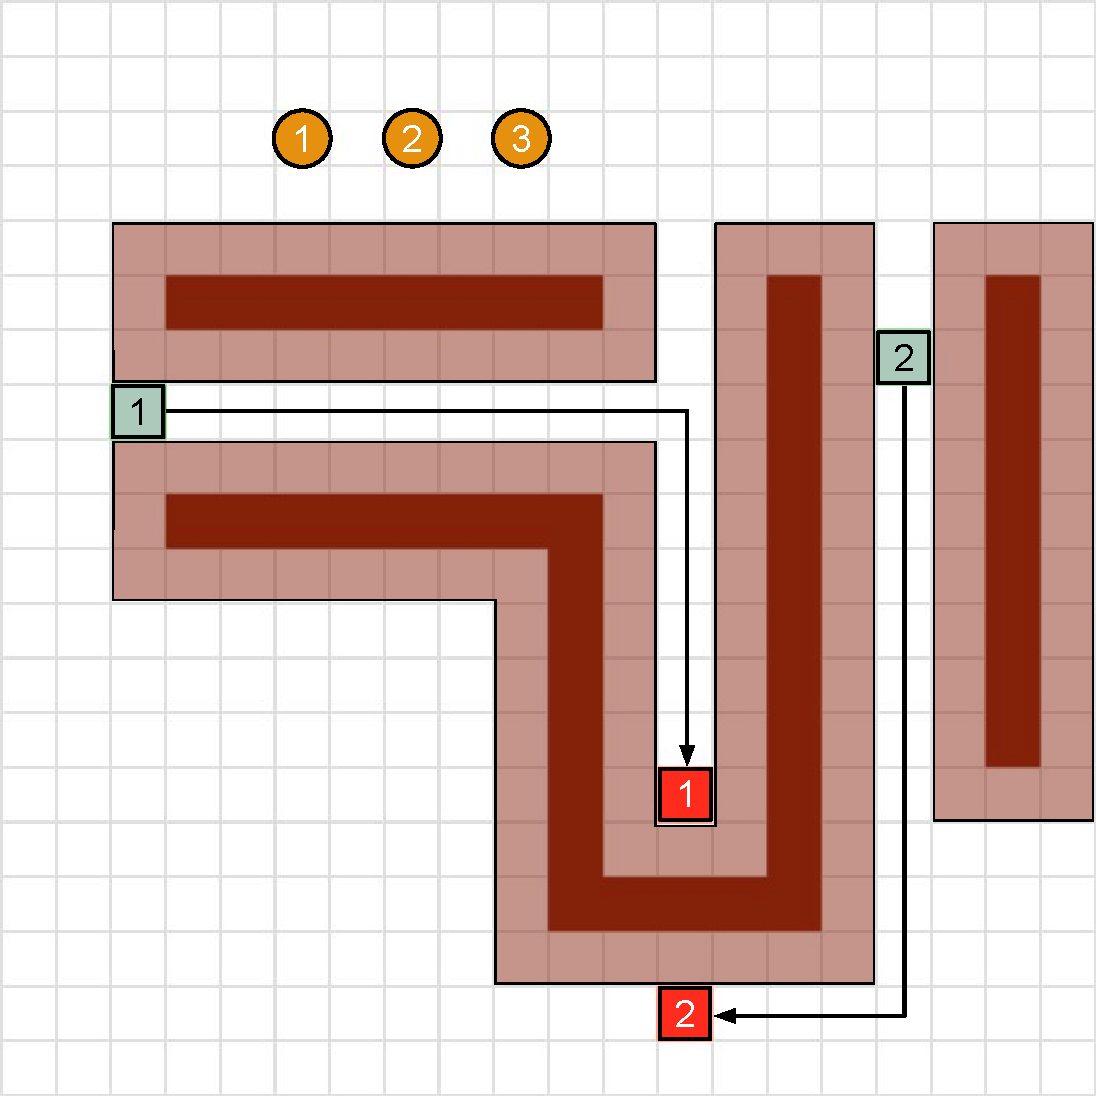
\includegraphics[width=0.8\textwidth]{img/execution/Mov1.pdf}}
    \caption{A etapa de planejamento para os objetos é executada.}
  \end{subfigure}
  \hspace{0.2cm}
  \begin{subfigure}[t]{0.45\textwidth}
    \centering
    \fbox{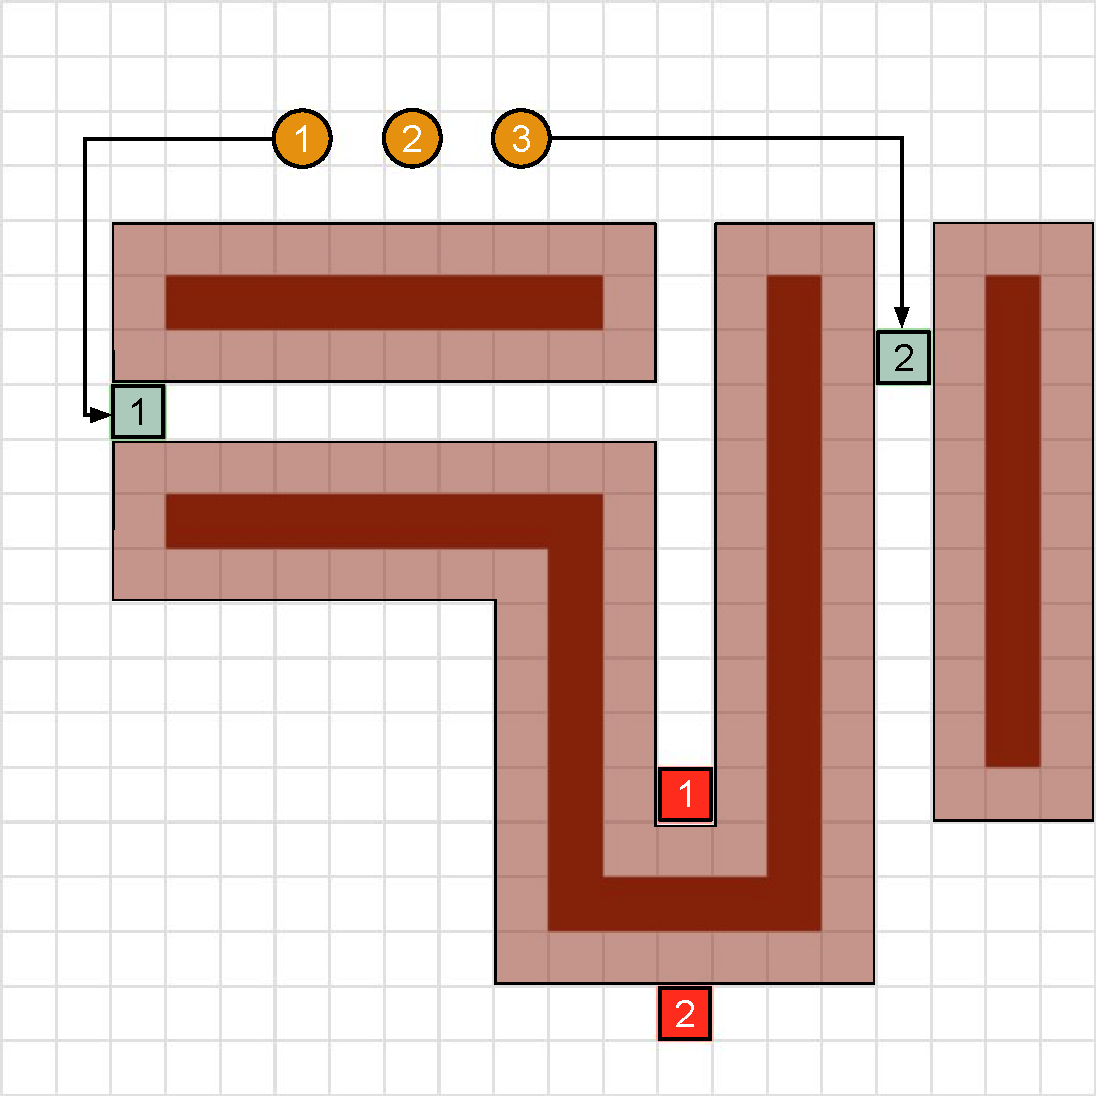
\includegraphics[width=0.8\textwidth]{img/execution/Mov2.pdf}}
    \caption{Pela proximidade dos objetos, os Agentes 1 e 3 são designados para os Objetos 1 e 3 respectivamente. Agente 2 não é alocado neste momento.}
  \end{subfigure}

  \vspace{0.3cm}
  \begin{subfigure}[t]{0.45\textwidth}
    \centering
    \fbox{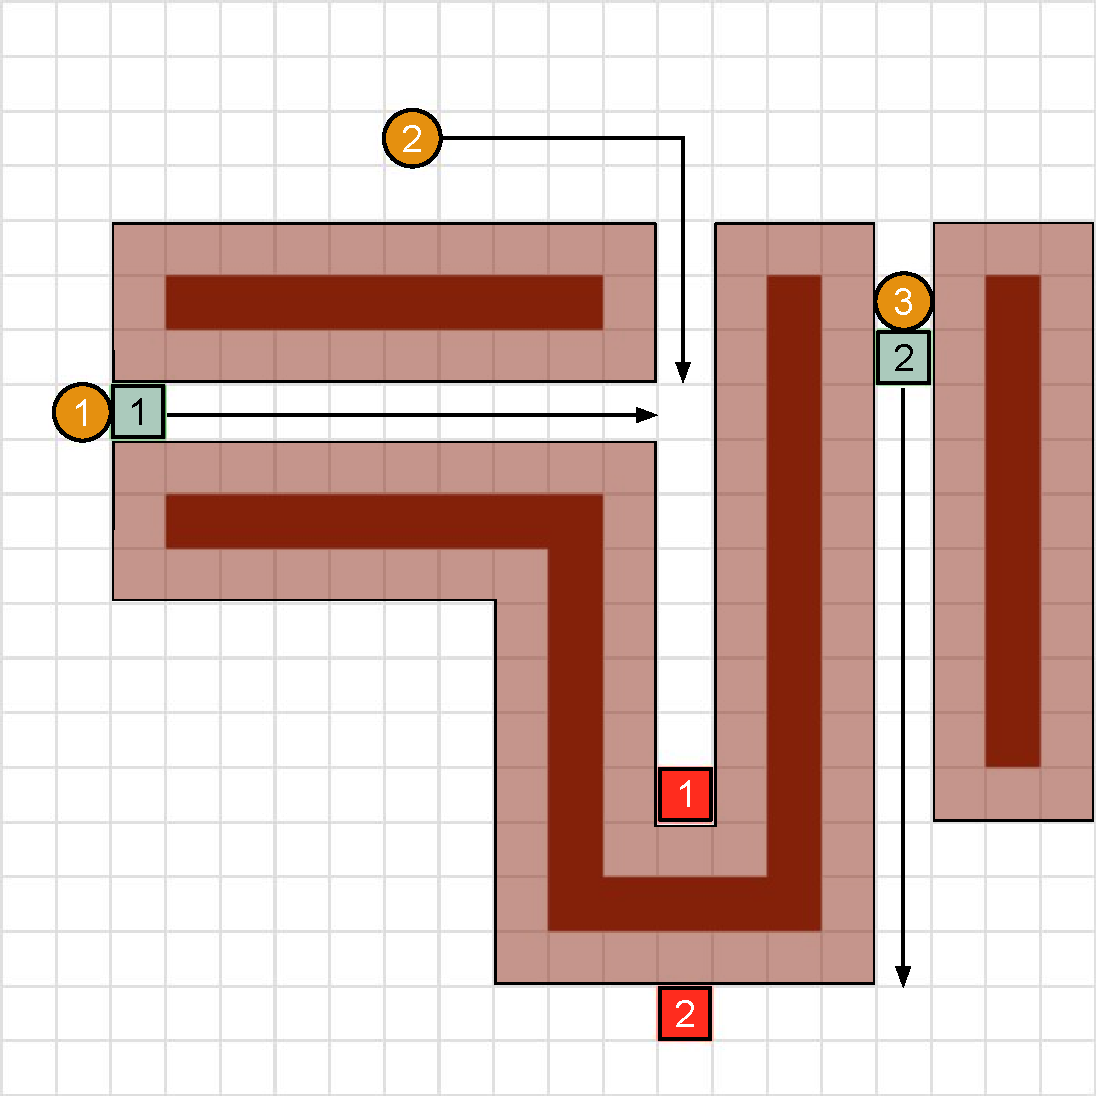
\includegraphics[width=0.8\textwidth]{img/execution/Mov3.pdf}}
    \caption{Plano de transporte é executado por cada agente em seu respectivo objeto.}
  \end{subfigure}
  \hspace{0.2cm}
  \begin{subfigure}[t]{0.45\textwidth}
    \centering
    \fbox{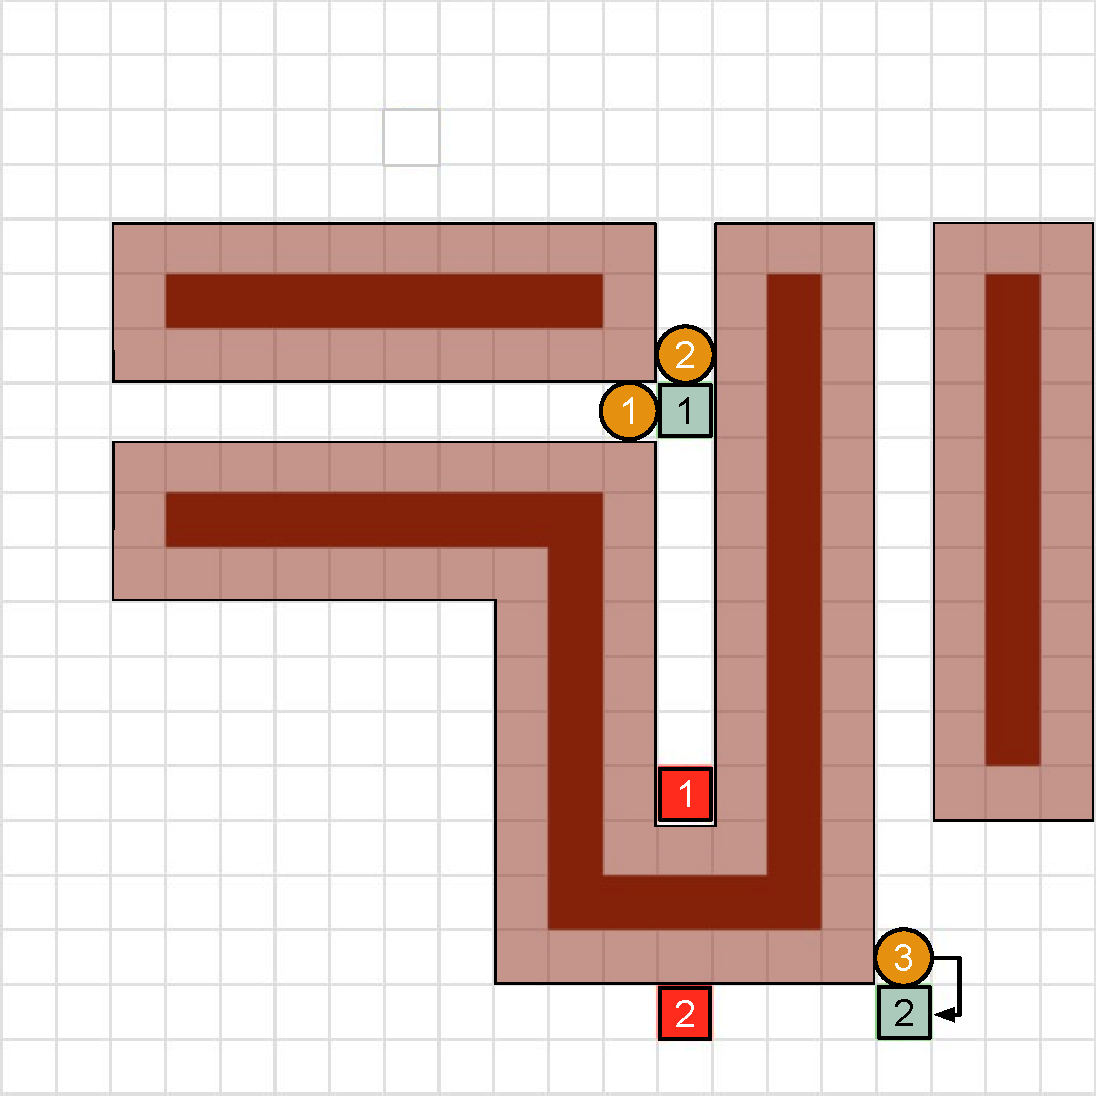
\includegraphics[width=0.8\textwidth]{img/execution/Mov4.pdf}}
    \caption{O agente 2 é alocado para o objeto 1, pois os demais agentes estão impossibilitados. Agente 3 continua responsável pelo objeto 2.}
  \end{subfigure}

  \vspace{0.3cm}
  \begin{subfigure}[t]{0.45\textwidth}
    \centering
    \fbox{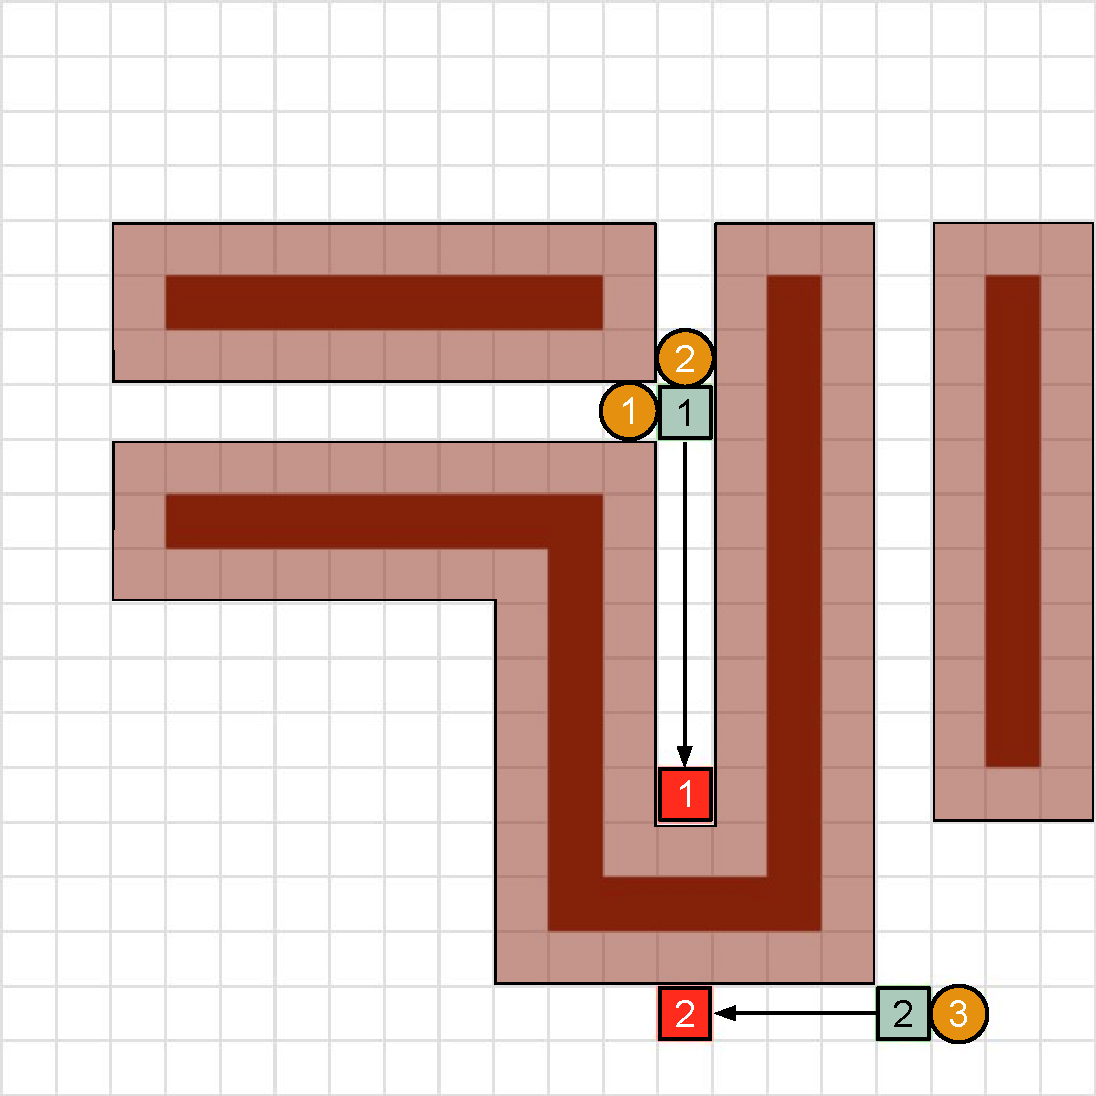
\includegraphics[width=0.8\textwidth]{img/execution/Mov5.pdf}}
    \caption{Agentes se aproximam dos objetos a serem transportados.}
  \end{subfigure}
  \hspace{0.2cm}
  \begin{subfigure}[t]{0.45\textwidth}
    \centering
    \fbox{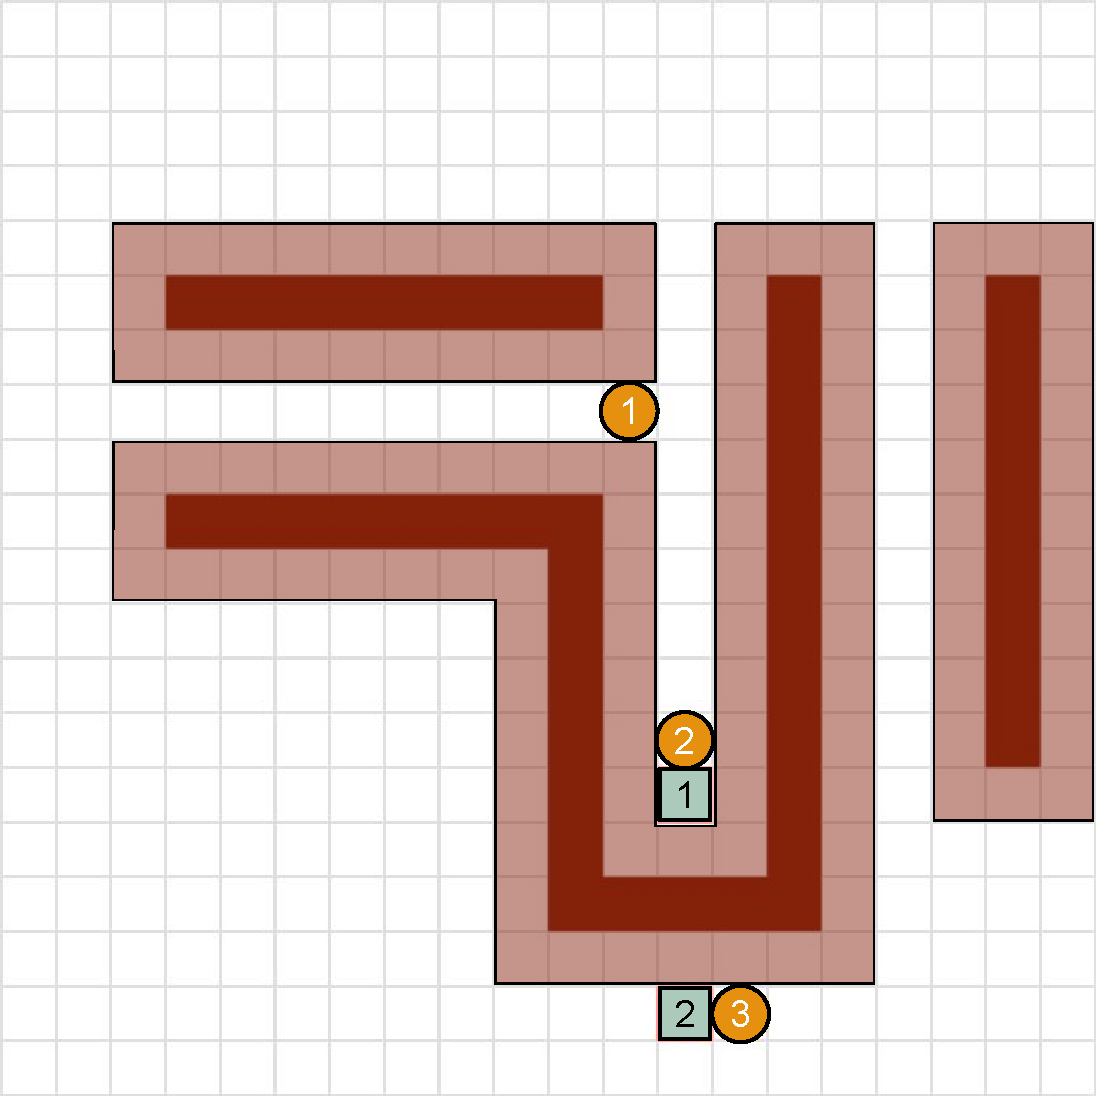
\includegraphics[width=0.8\textwidth]{img/execution/Mov6.pdf}}
    \caption{É realizada a movimentação final dos objetos para seus locais de destino.}
  \end{subfigure}

  \caption[Ambiente de exemplo com 2 objetos e 3 robôs]{Ambiente de Exemplo com 2 Objetos e 3 Robôs. É demonstrada a execução de todas as etapas da tarefa de transporte por uma equipe de agente autônomos.}
  \label{fig:execution_example}
\end{figure}

A Figura \ref{fig:execution_example} ilustra a execução da tarefa de transporte de objetos usando uma equipe de três agentes terrestres para manipular 2 objetos em um ambiente de exemplo. As etapas descritas na figura demonstram que o algoritmo de alocação considera principalmente a distância percorrida pelos agentes, pois no caso de uma equipe homogênea, somente esta dimensão é diferenciada entre os planos.

Como mencionado anteriormente, toda a etapa de planejamento e alocação das tarefas é executada antes que os agentes iniciem o processo de transporte, desta maneira cada agente já está ciente das tarefas que deve realizar.

\section{Coordenação} % (fold)
\label{sec:coordena_o}

Coordenação é a etapa de controle e ordenação de um processo para realização de uma tarefa ou atividade.
Para realizar o transporte de objetos por um equipe de agentes, os mesmos devem ser gerenciados de modo a executar suas tarefas na ordem correta e de forma coordenada.

Durante a execução do transporte, um objeto a ser transportado não pode ser manipulado por mais de um agente ao mesmo tempo, de modo que somente um agente esteja autorizado a realizar sua tarefa em uma dada fase do transporte.
O controle de autorização é feito mediante a troca de recursos nomeados \token, que são compartilhados pelos agentes.
Esta técnica é baseada no protocolo de comunicação de redes de computadores \emph{Token Ring}, no qual uma estrutura especial chamada \token\ circula pela rede, e somente o sistema que possuir tal informação é capaz de enviar dados pela rede.
No sistema implementado, existem várias estruturas \token, cada uma possui uma referência para um determinado objeto, que define a permissão para o agente.

Como mencionado na Seção \ref{sec:aloca_o_de_tarefas}, as tarefas a serem realizadas pelos agentes são os segmentos de cada objeto, de modo que para executar o segmento \segment{i+1}, o segmento antecessor \segment{i}\ deve ter sido completado anteriormente.
Esta precedência é válida e necessária em qualquer momento durante o transporte, pois um segmento futuro inevitavelmente não pode ser realizado, considerando que o objeto não estará na posição \originstate\ demarcada pelo mesmo.
Os segmentos são uma sequência de ações que devem ocorrer na forma ordenada que foram planejados e de nenhuma outra maneira.

O Algoritmo \ref{alg:coordination} é executado em cada agente do sistema e propõe o método de coordenação da equipe mediante a troca das estruturas \token, de modo a autorizar ou não algum agente a realizar suas tarefas para um determinado objeto.
Similar ao planejamento dos objetos, inicialmente um agente arbitrário possui todos os \token{s} de todos os objetos, e mediante a execução do algoritmo os mesmos são enviados e recebidos entre a equipe.

\begin{algorithm}
  \caption[CoordinationProcess]{CoordinationProcess(\tasklist)}
  \label{alg:coordination}

  \begin{algorithmic}[1]
    \LOOP
      \STATE{task $\leftarrow$ get\_first\_task(\tasklist)}

      \IF{ task $=$ NULL }
        \STATE{\textbf{break}}
      \ENDIF
      \STATE{}

      \IF{own\_token(task)}
        \STATE{\token\ $\leftarrow$ get\_token(task)}
      \ELSE
        \STATE{\token\ $\leftarrow$ request\_token(task)}
        \STATE{save\_token(\token)}
      \ENDIF

      \STATE{}
      \IF{ \NOT \token\ $=$ NULL }
        \STATE{execute\_prepare\_plan(task)}
        \STATE{execute\_transport\_plan(task)}
        \STATE{drop\_task(task)}
      \ENDIF

      \STATE{}
      \STATE{share\_ready()}
      \STATE{wait\_until\_reveice\_all\_ready()}

    \ENDLOOP
  \end{algorithmic}
\end{algorithm}

Após a etapa de alocação de tarefas, cada agente possui sua própria lista de tarefas \tasklist\ que deve completar.
No processo de coordenação, o agente executa ordenadamente suas tarefas utilizando a lista como uma fila, ou seja, as primeiras tarefas adicionadas também serão as primeiras a serem executadas.
A função \emph{get\_first\_task()} retorna a primeira tarefa seguindo este modelo de fila, ou retorna vazio (\emph{null}) se o agente não possuir mais tarefas a serem realizadas.

Uma vez com a tarefa selecionada, o agente testa se já possui o \token\ referente ao objeto a ser transportado (função \emph{own\_token()}), se possuir tal \token, o agente necessita recuperar de sua lista de \token{s}, caso contrário, realiza uma requisição para os demais agentes através da função \emph{request\_token()}, que será melhor explanado a seguir, pois um algoritmo de resposta deve ser executado nos agentes que recebem a requisição.
Quando a requisição for realizada com sucesso, o \token\ é transferido entre os agentes, e o robô o salva internamente (função \emph{save\_token()}).

Mediante o \token\ de autorização, o agente é capaz de realizar ambos os planos relacionados à tarefa, de preparação (\emph{execute\_prepare\_plan()}) e de transporte (\emph{execute\_transport\_plan()}). Após a execução destes passos, o agente pode descartar a tarefas e marcá-la como realizada (função \emph{drop\_task()}).

Neste momento, em que a tarefa atual foi realizada, o robô avisa aos demais agentes de seu estado (função \emph{share\_ready()}) e entra em modo de espera, até que toda a equipe informe o mesmo (função \emph{wait\_until\_reveice\_all\_ready()}).

Durante a execução das tarefas, os agentes realizam diversas trocas das estruturas \token, requisitando autorização para realizar suas próximas tarefas. Sempre que um agente realiza o pedido para a equipe, o Algoritmo \ref{alg:response_token} é executado de modo a processar o pedido.

O algoritmo recebe como parâmetro a tarefa vinda do outro agente (\emph{foreign\_task}), e realiza uma comparação com as suas próprias tarefas.
Se o agente no primeiro momento não possuir o \token\ referente ao objeto da tarefa externa, não há necessidade de realizar demais testes, e retorna vazio após o teste da função \emph{own\_token()}.

No caso em que o agente requisitado possuir o \token, o algoritmo é continuado realizando algumas validações na lista de tarefas \tasklist\ do mesmo.
Para cada tarefa da lista, dois dados são comparados:
(i) se ambas as tarefas (do agente e a tarefa externa) se referem ao mesmo objeto (função \emph{get\_object()}), e
(ii) se o teste anterior for verdadeiro, é testado se a tarefa possui um índice menor de segmento, ou seja, se a tarefa deve ser realizada antes da tarefa externa, neste caso, o agente não pode autorizar a realização da tarefa e retorna vazio (\emph{null}).
Na situação em que todas as tarefas do agente não atenderem esses testes, o mesmo disponibiliza seu \token\ para o agente requerente (função \emph{get\_token()}).

% \begin{description}
%   \item[get\_first\_task()] Durante o processo de alocação, as tarefas de responsabilidade de cada robô foram guardadas de forma ordenada. Esta função retorna a primeira tarefa ainda não realizada.
%   \item[request\_token(task)] O agente requisita aos demais agentes o \token\ para realização de sua tarefa. Este pedido é recebido pela equipe, e cada agente executa o processo descrito pelo Algoritmo \ref{alg:response_token}.
%   \item[execute\_move\_plan(task)] O robôs executa o plano de preparação para o transporte do objeto.
%   \item[execute\_transport\_plan(task)] É executado o plano de transporte do objeto.
%   \item[drop\_task(task)] O agente marca como executada a tarefa atual.
% \end{description}

\begin{algorithm}
  \caption[ResponseTokenProcess]{ResponseTokenProcess(foreign\_task)}
  \label{alg:response_token}

  \begin{algorithmic}[1]
    \STATE{\tasklist $\leftarrow$ get\_tasks()}
    \STATE{\object{f} $\leftarrow$ get\_object(foreign\_task)}
    \STATE{\segment{f} $\leftarrow$ get\_segment(foreign\_task)}

    \IF{\NOT own\_token(task)}
      \RETURN{NULL}
    \ENDIF

    \STATE{}
    \FORALL{task $\in$ \tasklist}
      \STATE{\object{i} $\leftarrow$ get\_object(task)}
      \STATE{\segment{i} $\leftarrow$ get\_segment(task)}

      \IF{\object{f} $=$ \object{i} \AND \segment{i} $<$ \segment{f}}
        \RETURN{NULL}
      \ENDIF
    \ENDFOR

    \RETURN{get\_token(\object{f})}

  \end{algorithmic}
\end{algorithm}

Ao considerar que mais de um agente pode mover-se ao mesmo tempo, e as rotas de movimentação podem se interceptar, durante a execução dos trajetos, os robôs mantém uma comunicação com os demais membros da equipe, informando sua posição atual e o plano que está executando.
Os agentes realizam testes de intersecção entre os planos que estão executando, e se for detectada uma eminente colisão, um sistema de prioridade é aplicado seguindo uma regra de maior distância, ou seja, mediante o tamanho do plano a ser executado (quantidade de passos a serem executados), o agente que possuir a menor tarefa deve esperar até que o outro robô envolvido no processo prossiga com seu plano.
Esta estratégia é exemplificada na Figura \ref{fig:priority}.

\begin{figure}[htpb]
  \centering
  \setlength{\fboxsep}{0pt}
  \begin{subfigure}[t]{0.45\textwidth}
    \centering
    \fbox{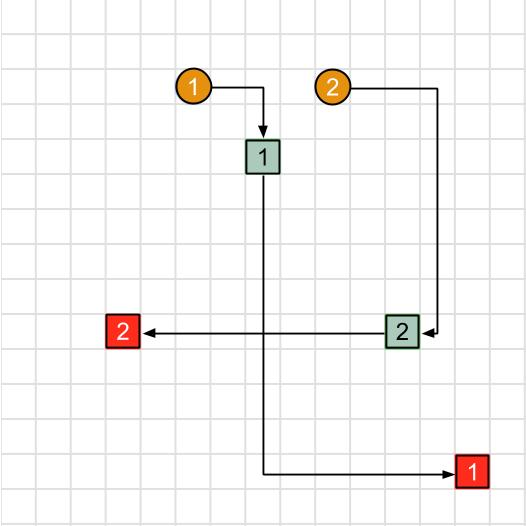
\includegraphics[width=0.8\textwidth]{img/coordination/Mov1.jpg}}
    \caption{Ambiente de Exemplo: 2 Objetos, 2 Robôs. É executado o planejamento para os objetos e a alocação. É demonstrado os planos de preparação dos robôs.}
  \end{subfigure}
  \hspace{0.2cm}
  \begin{subfigure}[t]{0.45\textwidth}
    \centering
    \fbox{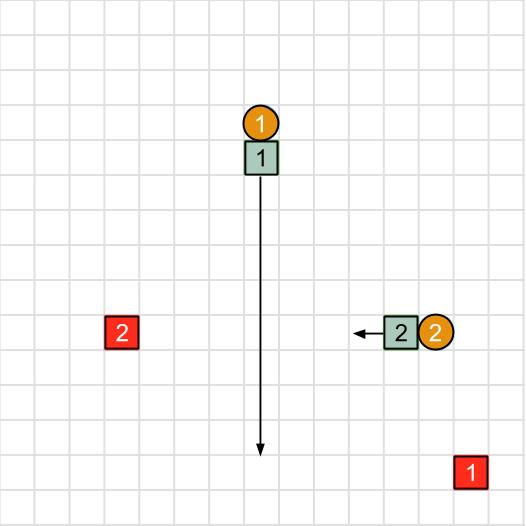
\includegraphics[width=0.8\textwidth]{img/coordination/Mov2.jpg}}
    \caption{Durante o transporte, é verificado que o plano do objeto 1 é maior, portanto tem prioridade sobre o objeto 2.}
  \end{subfigure}

  \vspace{0.3cm}
  \begin{subfigure}[t]{0.45\textwidth}
    \centering
    \fbox{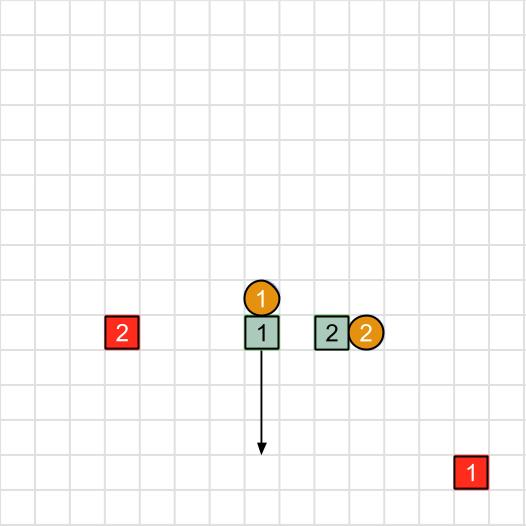
\includegraphics[width=0.8\textwidth]{img/coordination/Mov3.jpg}}
    \caption{O Agente 2 executa parte do plano total, e espera a passagem do outro robô.}
  \end{subfigure}
  \hspace{0.2cm}
  \begin{subfigure}[t]{0.45\textwidth}
    \centering
    \fbox{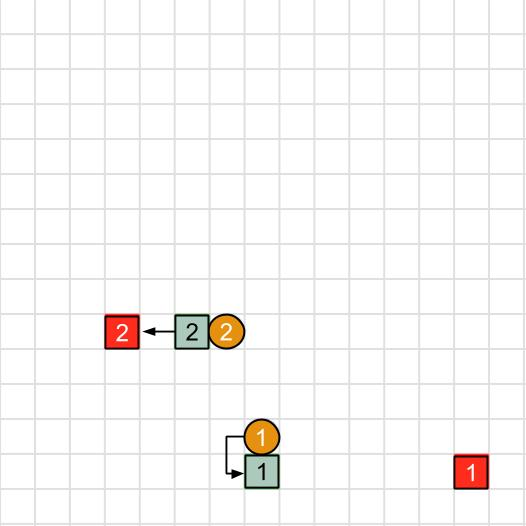
\includegraphics[width=0.8\textwidth]{img/coordination/Mov4.jpg}}
    \caption{Após o Agente 1 executar seu plano, o Agente 2 pode continuar o transporte do Objeto 2.}
  \end{subfigure}

  \vspace{0.3cm}
  \begin{subfigure}[t]{0.45\textwidth}
    \centering
    \fbox{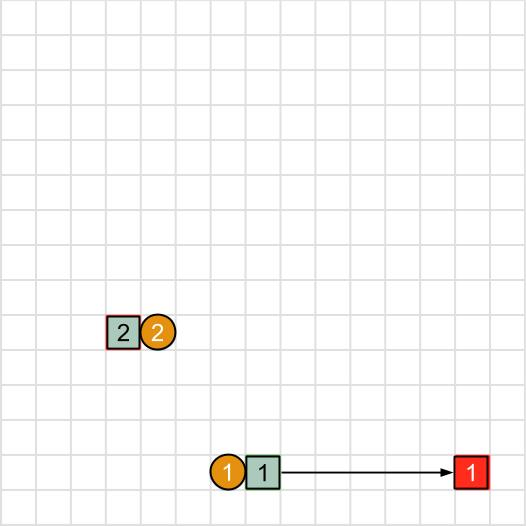
\includegraphics[width=0.8\textwidth]{img/coordination/Mov5.jpg}}
    \caption{Agente 2 finaliza o transporte. Agente 2 realiza o movimento de preparação.}
  \end{subfigure}
  \hspace{0.2cm}
  \begin{subfigure}[t]{0.45\textwidth}
    \centering
    \fbox{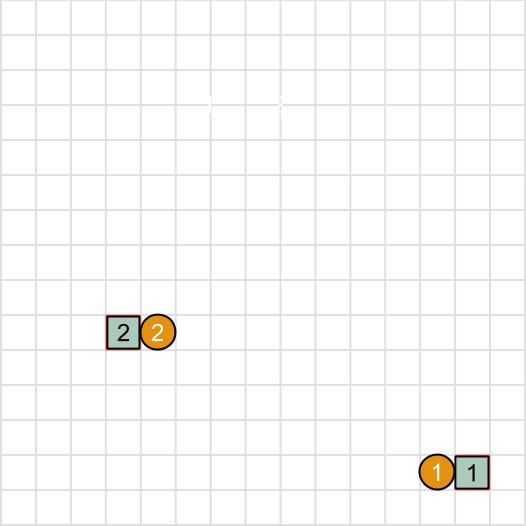
\includegraphics[width=0.8\textwidth]{img/coordination/Mov6.jpg}}
    \caption{O transporte de todos os objetos é concluído.}
  \end{subfigure}

  \caption[Exemplo de Coordenação entre 2 Agentes durante o transporte de objetos]{Exemplo de Coordenação entre 2 Agentes durante o transporte de objetos demonstrando a técnica aplicada quando há uma intersecção entre os planos de movimentação.}
  \label{fig:priority}
\end{figure}

\endinput

Como mencionado na Seção \ref{sec:aloca_o_de_tarefas}, cada tarefa dentro do sistema representa um plano \robotplan{i} $\in$ \robotplanset, que devem ser percorridos para executar o transporte.
O mecanismo de controle para que um determinado agente \robot{i} realize as tarefas que lhe foram atribuídas segue os seguintes passos:

\begin{enumerate}
  \item A ordem de execução das tarefas previamente distribuída entre os agentes é seguida considerando a sequência de segmentos do conjunto \segmentset;
  \item São criados \token\ do tipo $<$\movementtypepremove$>$ em quantidade igual aos segmentos do conjunto \segmentset, em seguida são adicionados ao conjunto \tokenset;
  \item É criado somente um (1) \token\ do tipo $<$\movementtypemove$>$ e é adicionado ao conjunto \tokenset.
  \item Para cada \segment{i}\ $\in$ \segmentset:
    \begin{enumerate}
      \item É dado ao agente responsável pelo segmento um (1) \token do tipo $<$\movementtypepremove$>$ e o \token\ do tipo $<$\movementtypemove$>$;
      \item Ao agente responsável pelo próximo segmento, se houver, é dado um (1) \token\ do tipo $<$\movementtypepremove$>$;
      \item Após a realização do plano do tipo $<$\movementtypepremove$>$, o \token\ é devolvido ao conjunto \tokenset;
      \item Os passos são repetidos até que o último segmento seja realizado.
    \end{enumerate}
\end{enumerate}

A criação de somente um (1) \token\ do tipo $<$\movementtypemove$>$ restringe a quantidade de agentes realizando o plano deste tipo, pois o objeto só é manipulado por um agente por vez.
A fim de agilizar o processo de transporte, o agente do próximo segmento ganha um \token\ do tipo $<$\movementtypepremove$>$, de modo que pode realizar a etapa de preparação, e esperar que o agente do segmento atual termine sua tarefa para assim assumir o transporte.

Utilizando a técnica descrita, os agentes são capazes de realizar suas ações de forma ordenada e em consenso, além de aproveitar a etapa que antecede o transporte em si para ganhar tempo durante todo o processo.
Esta etapa, a de execução da tarefa, é realizada através da comunicação e troca de informações entre os agentes, como o estado atual de suas ações e a troca e envio de \token\ dentre os mesmos.

% section coordena_o (end)

% chapter metodologia (end)
